    \documentclass[10pt]{article}
    \usepackage[dvips]{graphicx}
    \usepackage{alltt}
%    \usepackage{color}

    \newcommand*{\tc}{\ttfamily} % type computer
    \newcommand*{\tn}{\sffamily} % type names 
    \newcommand*{\p}{\partial} 
    \newcommand*{\ol}{\overline} 

    \pagestyle{headings}

    \begin{document} 
    
%///////////////////////////////////////////////////////////////////////
    \begin{titlepage}

    \begin{flushleft}
%- - - - - - - -%
% TU Delft logo %
%- - - - - - - -%
    \begin{figure}
    \includegraphics[scale=1.0]{tu_logo.eps}
    \end{figure}

    {\large\bf Delft University of Technology } \\
    {\large    Faculty of Applied Physics }\\
    {\large    Section: Thermal and Fluid Sciences} \\
    \end{flushleft}

    \vspace*{1.0cm}

    \begin{center}

    {\Huge \bf \tn T-Rex \\ }
    \vspace*{1.0cm}
    {\LARGE \tn User's Manual \\ }
    \vspace*{1.0cm}
    {\large \tn Version~2.0 \\ }
    {\large \tn \today \\ }

    \vspace*{2.0cm}

    {\large B. Ni\v{c}eno and K. Hanjali\'{c}}

    \vspace*{4.0cm}

    {\large\em Prepared for:} \\
    {\large    AVL-GmbH, Advanced Simulation Technologies }\\
    {\large    under the Contract: TN-96-033 } \\

    \end{center}
 

    \end{titlepage}
%///////////////////////////////////////////////////////////////////////

    \tableofcontents

%================================================================
%
    \newpage
    \section{Introduction}
%
%================================================================

    This manual describes the {\tn T-Rex} a software package 
    for calculation of unsteady three-dimensional laminar and 
    turbulent incompressible fluid flow. 
    
    {\tn T-Rex} consists of three principal programs: grid
    generator ({\tn Generator}), domain decomposer ({\tn Divisor})
    and the central program for calculation of the equations which
    describe the incompressible fluid flow
    ({\tn Processor}). All the principal programs are written in 
    Fortran~90
    programming language. {\tn Generator} and {\tn Divisor} can
    be used on the single processor computer only, whereas 
    {\tn Processor} can be used on both sequential and parallel
    computers. 

    In addition to this three principal programs, four 
    more utilities are added: {\tn F2html} for creating the 
    source code in HTML format for analysis and documentation,
    {\tn Connect} utility which connects the result files
    obtained from different processors (during the 
    parallel) execution into a single result
    file, {\tn A2B} and {\tn B2A} for converting some files
    created by {\tn T-Rex} from ASCII to binary format and
    vice versa. 
    {\tn F2html} and {\tn Connect} are written in the
    ANIS C~language, whereas {\tn A2B} and {\tn B2A} are
    written in Fortran~77.

    In the parallel version, the Message Passing
    Interface (MPI) library has been used for exchanging the 
    data between the processors.   

%------------------------------------------
    \subsection{{\tn Generator}}
%------------------------------------------
 
    {\tn Generator} is constrained to hexahedronal cells only.
    The grid can be refined by stretching the grid lines  
    and/or by locally splitting the cells in the regions of
    particular interest. Grid lines may be smoothed after the
    mesh generation, to avoid the sharp edged control volumes.
    However, it is not very user-friendly, and the generation
    of very complex domains may become very tedious and 
    cumbersome. The user is therefore advised to use it
    just for the demonstration purposes, and, if possible,
    to use some commercial and qualitative grid generator.
    This will require the development of some conversion 
    interface for the output files. The {\tn Generator} can 
    run only on a single processor computer.  The usage of the 
    {\tn Generator} is explained in more details in section
    (\ref{Gen})
    
%------------------------------------------
    \subsection{{\tn Divisor}}
%------------------------------------------

    {\tn Divisor} reads the output files created by 
    {\tn Generator} and divides the computational domain into 
    arbitrary number of sub-domains for subsequent parallel 
    computation.
    It is based on {\em geometrical multi section}. It is very
    efficient, and fully automatic. The user just has to
    enter the number of processors he would like to use, and
    {\tn Divisor} will automatically divide the domain into
    perfectly balanced sub-domains and save each sub-domain
    in a separate file for subsequent parallel processing.   
    If a user wants to run the simulation on a sequential 
    (single processor) computer, he/she can skip the usage of 
    {\tn Divisor}.

%------------------------------------------
    \subsection{{\tn Processor}}
%------------------------------------------

    {\tn Processor} is based on the second order
    accurate control volume (CV) numerical method on general, 
    unstructured grid. Grids of any topology are allowed, including
    locally refined and/or hybrid grids. Control volumes can have any
    shape, and arbitrary number of neighbours. The colocated
    variable arrangement is used, i.e.\ velocities and pressures
    are calculated in cell centres. Gradients of dependent
    variables are calculated using the least squares method, so
    there is no need for geometrical transformation on the cell
    faces. Several time-integration schemes may be used: fully
    implicit, semi-implicit Crank-Nicholson, explicit Adams-Bashforth.
    Different time-integration schemes can be used for different
    parts of the discretised system of equations, so the user can use
    Crank-Nicholson scheme for diffusive terms for stability 
    and Adams-Bashforth for convective and cross diffusive parts
    for simplicity. Velocities and pressure may be linked with
    the implicit SIMPLE procedure, or with explicit fractional
    step method.
    Since the main purpose of {\tn Processor} is large eddy simulation
    (LES) of turbulence, which is very demanding technique in 
    terms of computer memory and time, it has been parallelised
    by the domain decomposition technique. 
    
      
    
%------------------------------------------
    \subsection{Visualisation}
%------------------------------------------
    There is no program for visualisation included in the
    {\tn T-Rex} package. However, {\tn T-Rex} currently saves
    data in AVS (Unigraph), commercial visualisation package
    and GMV 
      \footnote{{\tc http://www-xdiv.lanl.gov/XCM/gmv/GMVHome.html}} 
    a free-ware visualisation package. If a user doesn't
    have access to AVS, he/she can download GMV at no charge and
    visualise grids and results with it. For the users convenience,
    the GMV executables for various platforms are included on
    the accompanying Zip drive. 

%================================================================
%
    \newpage
    \section{Contents of the {\tn T-Rex} package}
%
%================================================================

    {\tn T-Rex} is currently provided with:
    \begin{itemize}
      \item Zip drive containing:
        \begin{itemize}
          \item this manual in Postscript format {\tc Manual.ps}
          \item all the necessary source in {\tc T-Rex.tar.gz} archive,
          \item unpacked sources in {\tc T-Rex} directory,
          \item sources in HTML format in the {\tc HTML} directory,
          \item GNU make utility, versions 3.75 and 3.77 in the
                {\tc GNUmake} directory 
          \item GMV visualisation package for various computational
                platforms in the {\tc GMV} directory,
        \end{itemize}
      \item Floppy diskette with compressed sources in the file
            {\tc trex.tgz}. The floppy is included just in case
            the user don't have acces to the Zip drive. 
      \item This manual in printed format.  
    \end{itemize}

%================================================================
%
    \newpage
    \section{Compiling the {\tn T-Rex} package}
%
%================================================================

    Software requirements:
    \begin{itemize}
      \item Fortran~90 compiler 
            for compilation of principal
            programs ({\tn Generator}, {\tn Divisor} and {\tn Processor})
      \item ANSI C compiler for compilation of additional utilities
            ({\tn F2html} and {\tn Connect}),
      \item GNU make utility. 
    \end{itemize}
%
    So far, {\tn T-Rex} has been developed and tested on the following
    computing platforms:
    \begin{itemize}
      \item Intel PC running Linux (kernels 2.x and higher)
            with freeware Vast Fortran 90 compiler,
      \item Hewlett-Packard workstations running HP-UX versions
            A.09.01 and B.10.20, with FORTRAN~90 version~1.0, 
      \item Cray J90 running UNICOS version~10.0 with CF90~3.0,
      \item Cray C90 running UNICOS version~10.0.0.2 with CF90~3.1,
      \item Cray T3E running UNICOS/mk version~2.03 with CF90~3.1.0.0
    \end{itemize}

%----------------------------------------
    \subsection{Compiling the GNU make}
%----------------------------------------

    The first step is the instalation of the GNU~make utility on
    your system. If you already have the GNU~make on your 
    system, you can skip this section. For convenience,
    a GNU~make versions~3.75 and 3.77 are shipped with {\tn T-Rex} 
    package.
    The compilation of GNU~make is, from author's experience
    quite straightforward. The details of instalation are in the
    accompanying INSTALL file, but in general, it shouldn't be
    more difficult then unpacking the {\tc make-3.75.tar.gz} archive,
    going to directory {\tc make-3.75} and typing:
    \begin{alltt}
    ./configure
    make 
    make check
    \end{alltt}
    the executable for GNU~make, called {\tc make} will then reside 
    in the {\tc make-3.75} directory. You are advised to rename it to
    {\tc gmake} or {\tc gnumake} to distinguish it from the
    normal make and put it in your path.
 
%------------------------------------------
    \subsection{Compiling the {\tn T-Rex}}
%------------------------------------------

    When you are sure that GNU~make is available on your system,
    you can compile the {\tn T-Rex} package. The entire package
    is in the archive {\tc T-Rex.tar.gz}. 
    After unpacking the archive, the following directory 
    structure will appear:    
    \begin{description}
    \item[{\tc T-Rex/Doc}] contains frequently asked questions
          FAQ and README file, and two additional 
          sub-directories: 
       \begin{description}
       \item[{\tc T-Rex/Doc/HTML}] with sources in HTML format
       \item[{\tc T-Rex/Doc/LaTeX}] with documentation in .tex and .ps format.
       \end{description} 
    \item[{\tc T-Rex/Gen}] with sources and {\tc Makefile} for the {\tn Generator}
    \item[{\tc T-Rex/Div}] with sources and {\tc Makefile} for the {\tn Divisor} 
    \item[{\tc T-Rex/Pro}] with sources and {\tc Makefile} for the {\tn Processor}a
    \item[{\tc T-Rex/Lib}] with sources for libraries, i.e.\ modules shared
          by all the principal programs and some utilities,
    \item[{\tc T-Rex/Seq}] with sources specific for sequential execution,
    \item[{\tc T-Rex/Par}] with sources specific for parallel execution,
    \item[{\tc T-Rex/Test}] example problems and sources for utilities:
          {\tn Connect}, {\tn B2A} and {\tn A2B} 
    \end{description}
    Before starting the compilation, you must set the {\tc TARGET}
    environment variables to one of the following values
     \footnote{Just a reminder: if you are using csh you must set: 
               {\tc setenv TARGET linux} in your {\tc .cshrc} file, and if 
               you are using {\tc bash}, you must set {\tc export TARGET=linux}
               in your {.bashrc} file}:
    \begin{itemize} 
    \item {\tc linux} if you are compiling on the Linux operating
          system,
    \item {\tc hp} if you are compiling on the HP-UX operating
          system,
    \item {\tc cray-t3e} if you are compiling on the \mbox{Cray-T3E}.
    \end{itemize} 
    To compile each of the principal programs ({\tn Generator}, 
    {\tn Divisor} or {\tn Processor} you have to go to the 
    corresponding sub-directory ({\tc Gen}, {\tc Div} and {\tc Pro}
    and type:
    \begin{alltt}
    gmake 
    \end{alltt}
    on the command prompt. This will make an executable named {\tc RUN}   
    in the sub-directory you are in. If, however, you want to give
    more meaningful names to basic programs, you can type 
    (for example):
    \begin{alltt}
    gmake PROGRAM=Generator 
    \end{alltt}
    in the {\tc Gen} sub-directory, to have your mesh generator
    called {\tc Generator}. You can do similar in other directories
    where basic programs are ({\tc Div} and {\tc Pro}).

    To compile utilities {\tn Connect}, {\tn A2B} and {\tn B2A},
    go to {\tc Test} sub-directory and type:
    \begin{alltt}
    gmake connect  
    \end{alltt}
    to compile {\tn Connect} or:
    \begin{alltt}
    gmake convert  
    \end{alltt}
    to compile {\tn A2B} and {\tn B2A} utilities. 

    When you finish your work with {\tn T-Rex}, you can clean
    the mess on the disk by typing:
    \begin{alltt}
    gmake clean  
    \end{alltt}
    in each of the directories: {\tc Gen}, {\tc Div}, {\tc Pro}
    to remove all the object and executable files. Typing 
    the {\tc gmake clean} in the {\tc Test} directory will
    clean all the object and executables, plus all the grids
    in AVS, GMV or .eps format and all the restart files. 

%--------------------------------------------------
    \subsection{Compiling the {\tn F2html} utility}
    \label{Com}
%-------------------------------------------------

    {\tn F2html} is a program which takes the Fortran sources
    and converts them into html format. The sources in html
    format has highlighted syntax and links to user defined
    functions and subroutines. It also generates the {\em call`by} 
    view and {\em invocation view}.

    To compile the {\tn F2html} program, first unpack the 
    {\tc F2html.tar.gz} archive. Then go to the directory 
    {\tc F2html} and type {\tc gmake}. This will compile all
    the necessary files and create an executable file called
    {\tc F2html} in the current directory. You can put the
    executable in your path, for convenience.

%================================================================ 
%
    \newpage
    \section{Using {\tn T-Rex}}
%
%================================================================

    Usage of {\tn T-Rex} can be summarised in the following steps
    \begin{itemize}
      \item Generation of the computational grid with 
            {\tn Generator},
      \item (optional) partitioning the grid with {\tn Divisor}
            if the user wants to run the program in parallel
      \item Running the CFD simulation with {\tn Processor},
      \item (optional) connecting the result files from
            different processors (if {\tn Processor}) was run
            in parallel,
      \item visualisation of results. 
    \end{itemize}

%================================================================
%
    \subsection{Using {\tn Generator}}
    \label{Gen}
%
%================================================================

    {\tn Generator} is used to divide the problem domain into 
    a finite number of cells, or control volumes. As an input
    it takes a special ASCII file, so called the {\em domain file},
    which gives the instructions to {\tn Generator} how to generate
    the mesh. The domain file must be named as {\tc $<$NAME$>$.d}
    where {\tc $<$NAME$>$} is any string allowed by the operating
    system, whereas {\tc .d} is obligatory extension.
    As the output, {\tn Generator} gives the following:
    \begin{itemize}
      \item {\tc $<$NAME$>$.inp} - ASCII format; grid in AVS data 
            format, used for
            visualisation and optionally later partitioning of the
            grid,
      \item {\tc $<$NAME$>$.gmv} - ASCII format; grid in GMV data format, used
            only for later visualisation,
      \item {\tc $<$NAME$>$.cns} - binary format; topology of
            the grid and boundary condition markers,
      \item {\tc $<$NAME$>$.geo} - binary format; geometrical
            quantities: cell volumes, cell centre coordinates etc.\,
      \item {\tc $<$NAME$>$.x.eps}, {\tc $<$NAME$>$.y.eps}, {\tc $<$NAME$>$.z.eps}
            Encapsulated Postscript cuts through the domain for
            quick visualisation of the generated grid,
      \item {\tc $<$NAME$>$.eps},
            Encapsulated Postscript showing the shaded 3D view of the 
            grid. 
            quick visualisation of the generated grid.
    \end{itemize}

%-----------------------------------------------
    \subsubsection{Running the {\tn Generator}}
%-----------------------------------------------
    Compilation of {\tn Generator} is explained in section {\ref{Com}}.
    When the executable file for {\tn Generator} is created, the user
    has to go to the directory where the domain file resides and run
    it.
    When the {\tn Generator} starts, it writes it's logo on the screen
    and prompts the user with the
    following question:
    \small
    \begin{verbatim}
    Input problem name:
    \end{verbatim}
    \normalsize
    At this point user has to enter the name of the domain file
    ({\tn $<$NAME$>$}) {\em without} extension. {\tn Generator} will
    continue to work and will write some messages on the standard
    output. When it finishes the generation of the grid, it will
    prompt the user with following questions: 
    \small
    \begin{verbatim}
     Enter the x coordinate for cutting: 
     Enter the y coordinate for cutting: 
     Enter the z coordinate for cutting: 
    \end{verbatim}
    \normalsize
    The user has to enter the position of cutting planes in $x$,$y$
    and $z$ directions to each of these questions. Those planes 
    are used just for
    creation of Encapsulated Postscript cuts of the domain. 
    Finally, the {\tn Generator} will prompt the user with
    the question:
    \small
    \begin{verbatim}
     Enter the x, y and z coordinate of the camera: 
    \end{verbatim}
    \normalsize
    To that question user has to enter three numbers which
    are the $x$, $y$ and $z$ coordinates of the viewpoint
    (camera). This, camera position, will be used in the
    creation of the 3D figure in Encapsulated Postscript
    format. Note that the camera coordinate is also the
    source of light and be careful to place the camera
    outside the domain. 

%----------------------------------------------------------
    \subsubsection{Creating the domain file}
%----------------------------------------------------------
    Domain file consists of following sections, and all of them
    (except the comments) must be present in the file:
    \begin{itemize}
    \item[1.] Memory requirements - defines maximal number of nodes
              (and cells)
    \footnote{For xexahedronal cells, then number of cells is just 
              slightly smaller then the number of nodes. Therefore
              the memory for nodes and cells is allocated with a single
              constnt.}, 
              boundary cells and cell faces.  
    \item[2.] Points - defines number of points and their x, y and
              z coordinates
    \item[3.] Blocks - defines hexahedronal blocks. Each block is 
              defined with 8 points from the above list of points.
              It also defines the resolution of each block and it's
              weight in local i, j and k direction respectively.
    \item[4.] Lines - defines distribution of points on the lines
              weather by explicitly defining coordinates of each 
              point on th line, or by setting the weight of the line.
    \item[5.] Surfaces - defines weight of each surface.
    \item[6.] Boundary conditions - defines boundary markers for later
              insertion of boundary conditions.
    \item[7.] Periodic boundaries - defines periodic boundaries.
    \item[8.] Copy boundaries - defines copy boundaries.
    \item[9.] Refinement - defines regions of local refinement by 
              cell splitting. It can define rectangular, ellipsoidal
              region or region defined by a plane. 
    \item[10.] Smoothing - defines the region for Laplacian smoothing
              of the domain. 
    \item Comments - each line which begins with a character {\tc \#}
          or {\tc \%} is regarded as a comment line and skipped by the
          {\tn Generator}. Comment lines can appear anywhere in the
          input file.
    \end{itemize}

    The templated format of the domain file follows. The numbers on
    the left corresponds to the above descriptions, and are not part
    of the input file. Entities in this {\tc <>} brackets are variables,
    whereas entities in this {\tc ><} brackets denote keywords. A
    list of allowed keywords is enclosed in this {\tc[,,]} brackets
    and is separated by commas. Entities entered without any brackets
    are obligatory, and cannot be altered. The same nomenclature
    rules apply as well to description of all the other file formats
    in this manual. 
    \small
    \begin{alltt}
    1. <max_nodes>  <max_boundary_cells>  <max_cell_faces> 
    2. <num_points> 
            <point_id 1>  <x>  <y>  <z>
               . 
               .
               .
            <point_id num_points>  <x>  <y>  <z>
    3. <num_blocks> 
            <block_id 1>   <num_i>  <num_j>  <num_k>    
               <weigth_i>  <weigth_j>  <weigth_k> 
               <block_point 1> ... <block_point 8>
               .
               .
               .
            <block_id num_blocks>   <num_i>  <num_j>  <num_k>    
               <weigth_i>  <weigth_j>  <weigth_k> 
               <block_point 1> ... <block_point 8>
    4. <num_lines>  
            <line_id 1>  <line_point 1>  <line_point 2> 
               <node_id 1>  <x>  <y>  <z>
               .
               .
               .
               <node_id num_nodes>  <x>  <y>  <z>
             [OR]
           -<line_id 1>  <line_point 1>  <line_point 2> 
               <weigth> 
               . 
               .
               .
            <line_id num_lines>  <line_point 1>  <line_point 2> 
               <node_id 1>  <x>  <y>  <z>
               .
               .
               .
               <node_id num_nodes>  <x>  <y>  <z>
             [OR]
           -<line_id num_lines>  <line_point 1>  <line_point 2> 
               <weigth> 
    5. <num_surfaces> 
            <surface_id 1>  <surf_point 1> ... <surf_point 4>
               <weigth_i>  <weigth_j>  <weigth_k> 
               .
               .
               . 
            <surface_id num_surfaces>  <surf_point 1> ... <surf_point 4>
               <weigth_i>  <weigth_j>  <weigth_k> 
    6. <num_bc> 
            <bc_id 1> <i_start> <j_start> <k_start> <i_end> <j_end> <k_end>
               <block_id>  <marker>
            [OR]  
            <bc_id 1>  >position<  [IMIN,IMAX,JMIN,JMAX,KMIN,KMAX]  
               <block_id>  <marker>
               .
               .
               . 
            <bc_id num_bc> <i_start> <j_start> <k_start> <i_end> <j_end> <k_end>
               <block_id>  <marker>
            [OR]  
            <bc_id num_bc> >position< [IMIN,IMAX,JMIN,JMAX,KMIN,KMAX]   
               <block_id>  <marker>
    7. <num_per> 
            <per_id 1>  <point_surf_1 1> ... <point_surf_1 4> 
                        <point_surf_2 1> ... <point_surf_2 4> 
               .
               .
               . 
            <per_id num_per>  <point_surf_1 1> ... <point_surf_1 4> 
                              <point_surf_2 1> ... <point_surf_2 4> 
    8. <num_copy> 
            <copy_id 1>  <point_surf_1 1> ... <point_surf_1 4> 
                         <point_surf_2 1> ... <point_surf_2 4> 
               .
               .
               . 
            <copy_id num_per>  <point_surf_1 1> ... <point_surf_1 4> 
                               <point_surf_2 1> ... <point_surf_2 4> 
    9. <num_levels> 
            <level_id 1>  <num_regions>
               <region_id 1>  >shape<  [RECTANGLE,PLANE,ELIPSOID]  
                   <x1>  <y1>  <z1>  <x2>  <y2>  <z2>
               . 
               .
               .
               <region_id num_regions>  >shape<  [RECTANGLE,PLANE,ELIPSOID] 
                   <x1>  <y1>  <z1>  <x2>  <y2>  <z2>
            <level_id num_levels>  <num_regions>
               <region_id 1>  >shape<  [RECTANGLE,PLANE,ELIPSOID]  
                   <x1>  <y1>  <z1>  <x2>  <y2>  <z2>
               . 
               .
               .
               <region_id num_regions>  >shape<  [RECTANGLE,PLANE,ELIPSOID]  
                   <x1>  <y1>  <z1>  <x2>  <y2>  <z2>
    \end{alltt}
    \normalsize
    So far, we have introduced several issues which demand
    further explanation. Here we mean the weights, boundary
    conditions, refinement levels. We believe that they are
    best explained with few examples which now follow.

%------------------------------------------
    \paragraph{Example 1: A cavity}
%------------------------------------------

    We begin with probably the simplest possible test case
    which is the lid driven cavity flow. This example 
    illustrates the following:
    \begin{itemize}
    \item definition of a simple, single-block domain,
    \item definition of boundary condition markers,
    \item local cell refinement.  
    \end{itemize}
    The domain of interest is shown in figure~(\ref{cavity}).
%%%%%%%%%%%%%%%%%%
    \begin{figure}
%%%%%%%%%%%%%%%%%%
    \centering
    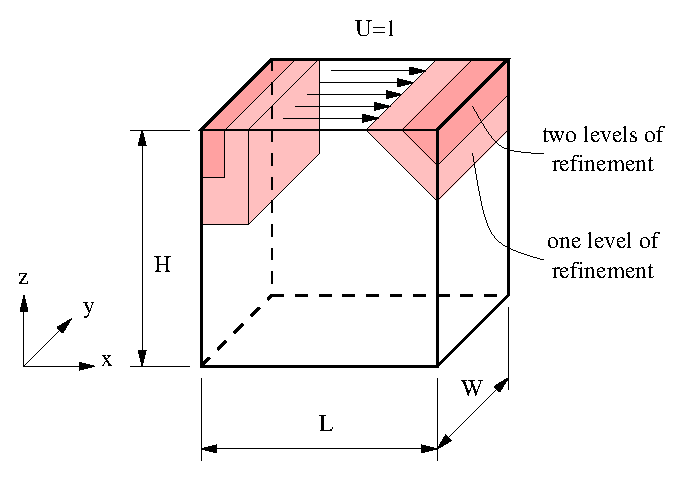
\includegraphics[scale=0.8]{cavity.eps}
    \caption{Problem domain for the cavity flow}
    \label{cavity}
    \end{figure}
%%%%%%%%%%%%%%%%%%
     Let's set the dimension of the domain to 
     $L \times W \times H = 1 \times 1 \times 1$, and let's 
     define two levels of local grid refinement in the regions 
     where high gradients of pressure can be expected. A regions
     with one level of refinement is emphasised in light gray 
     and regions with two levels of
     refinement are emphasised with dark gray in figure~(\ref{cavity}).
     Three different types of boundary conditions are required:
     prescribed velocity, wall and symmetry. At this stage, however,
     it is enough to know that three boundary markers are needed. 

     Each block is defined by it's local coordinate system ($i$,$j$,$k$),
     and local points. The correspondence between them is 
     illustrated
     in figure~(\ref{local}). In this case, local point numbers
     coincide with global numbers.
%%%%%%%%%%%%%%%%%%
    \begin{figure}
%%%%%%%%%%%%%%%%%%
    \centering
    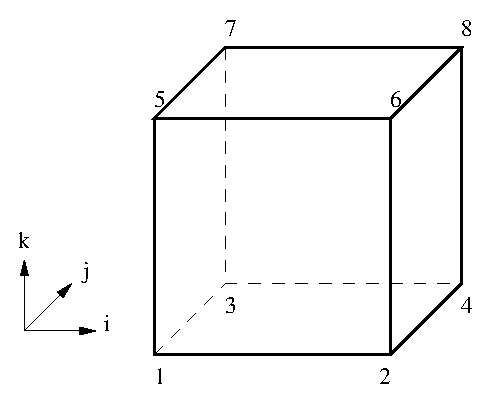
\includegraphics[scale=0.8]{local.eps}
    \caption{Problem domain for the cavity flow}
    \label{local}
    \end{figure}
%%%%%%%%%%%%%%%%%%

     The domain file begins with section for memory allocation. Maximal number
     of nodes (and cells), boundary cells and cell faces has to be given. For
     a locally driven cavity shown in figure~(\ref{cavity}), we might expect
     $30000$ nodes. A good rule of thumb says that it is necessary to reserve the
     one third of number of nodes for boundary cells and three times 
     the number of nodes for cell faces. Therfore, the section for memory  
     \small
     \begin{verbatim}
     #-------------------------------------------#
     #  Nodes (cells), boundary cells and sides  #
     #-------------------------------------------#
       30000 10000 90000
     \end{verbatim}
     \normalsize

     The domain file continues with
     section for points, which is nothing more then a list of
     points with their corresponding $x$, $y$ and $z$ coordinates:
     \small
     \begin{verbatim}
     #----------#
     #  Points  #
     #----------#
       8
         1   0.0   0.0   0.0
         2   1.0   0.0   0.0
         3   0.0   1.0   0.0
         4   1.0   1.0   0.0
         5   0.0   0.0   1.0
         6   1.0   0.0   1.0
         7   0.0   1.0   1.0
         8   1.0   1.0   1.0
     \end{verbatim}
     \normalsize
     This is followed by a section for blocks. In this case,
     only one block is defined:
     \small
     \begin{verbatim}
     #----------#
     #  Blocks  #
     #----------#
       1
         1  11   11   11
            1.0  1.0  1.0
            1  2  3  4  5  6  7  8
     \end{verbatim}
     \normalsize
     It is important to note that the initial grid will 
     have $11 \times 11 \times 11$ nodes which means 
     $10 \times 10 \times 10$ cells. Further, weights
     in all three local directions (i, j and k) are 
     equal to one, which means that no stretching of the
     grid lines will be performed. 
     In this case, we will not define anything special for
     lines and surfaces, so this two sections look like:
     \small
     \begin{verbatim}
     #---------#
     #  Lines  #
     #---------#
       0
     #------------#
     #  Surfaces  #
     #------------#
       0
     \end{verbatim}
     \normalsize
     After surface section, we came to boundary conditions,
     which looks like:
     \small
     \begin{verbatim}
     #-----------------------#
     #  Boundary conditions  #
     #-----------------------#
       3
         1     Kmax
               1   2
         2     Jmin
               1   3
         3     Jmax
               1   3
     \end{verbatim}
     \normalsize
    This section needs special attention. Three surfaces are 
    marked, the top surface ({\tc KMAX}) for prescribed velocity
    with marker 2, and two surfaces for symmetry boundary
    conditions with marker 3. {\em All the remaining surfaces,
    which are not defined in this section, will have the 
    default marker 1}. 
    There are no periodic boundary conditions, so the 
    section for them looks similar to one for lines and
    surfaces:
    \small
    \begin{verbatim}
    #-----------------------#
    #  Periodic boundaries  #
    #-----------------------#
      0                                
    \end{verbatim}
    \normalsize
    Copy boundaries are not present neither, therefore the section for copy
    boundaries looks like:
    \small
    \begin{verbatim}
    #-------------------#
    #  Copy boundaries  #
    #-------------------#
      0                                
    \end{verbatim}
    \normalsize
    Now follows the section for local cell refinement. As it
    was shown in figure/~(\ref{cavity}), we have two levels 
    of refinement, and each of them has two refined regions:
    a rectangle-shaped one in the upper right
    and the triangular-shaped one in the upper right corner of the
    domain. Rectangular regions are defined with keywords: {\tc FILL}
    and {\tc RECTANGLE} and six real numbers which represent x, y 
    and z coordinate of the lower-left-front and $x$, $y$ and $z$
    coordinates of the upper-right-back corner of the domain. A
    rectangular region is illustrated in figure~(\ref{rectangle}).   
%%%%%%%%%%%%%%%%%%
    \begin{figure}
%%%%%%%%%%%%%%%%%%
    \centering
    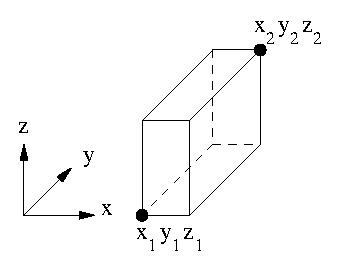
\includegraphics[scale=0.8]{rectangle.eps}
    \caption{Definition of rectangular region for refinement}
    \label{rectangle}
    \end{figure}
%%%%%%%%%%%%%%%%%%
    Triangular regions are defined with {\tc FILL} and {\tc PLANE}
    keywords and six more real numbers. First three numbers are
    the coordinates of the point belonging to that plane and the
    three remaining ones define the normal of the plane in the
    direction in which the refinement will take place. 
      \footnote{Apart from {\tc RECTANGLE} and {\tc PLANE} a keyword
      {\tc ELIPSOID} can also be used. If used it is also followed
      by six real numbers, where first three are the coordinates 
      of the ellipsoid centre, and the three remaining ones are 
      its principal axes in $x$, $y$ and $z$ direction.} 
    A planar region is illustrated in figure~(\ref{plane}).
%%%%%%%%%%%%%%%%%%
    \begin{figure}
%%%%%%%%%%%%%%%%%%
    \centering
    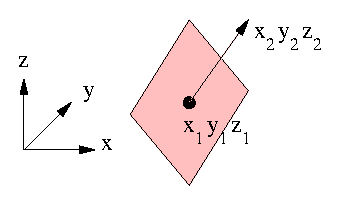
\includegraphics[scale=0.8]{plane.eps}
    \caption{Definition of planar region for refinement}
    \label{plane}
    \end{figure}
%%%%%%%%%%%%%%%%%%
    \small
    \begin{verbatim}
    #------------#
    # Refinement #
    #------------#
      2
    # level 1 #
        1  2
           1 Fill Rectangle
             0.0  0.0  0.6  0.2  1.0  1.0
           2 Fill Plane
             0.75 0.75 0.75 1.0  0.0  1.0
    # level 2 #
        2  2
           1 Fill Rectangle
             0.0  0.0  0.8  0.1  1.0  1.0
           2 Fill Plane
           0.85 0.85 0.85 1.0  0.0  1.0
    \end{verbatim}
    \normalsize
    The domain file finishes with smoothing section. For this
    domain, no smoothing is needed, so we just have to set 
    the number of smoothing regions to 0.
    \small
    \begin{verbatim}
    #-----------#
    # Smoothing #  
    #-----------#
      0
    \end{verbatim}
    \normalsize
    The final grid for this example is shown on figure~(\ref{cavfinal_p10_m30_p10}).
%%%%%%%%%%%%%%%%%%
    \begin{figure}
%%%%%%%%%%%%%%%%%%
    \centering
    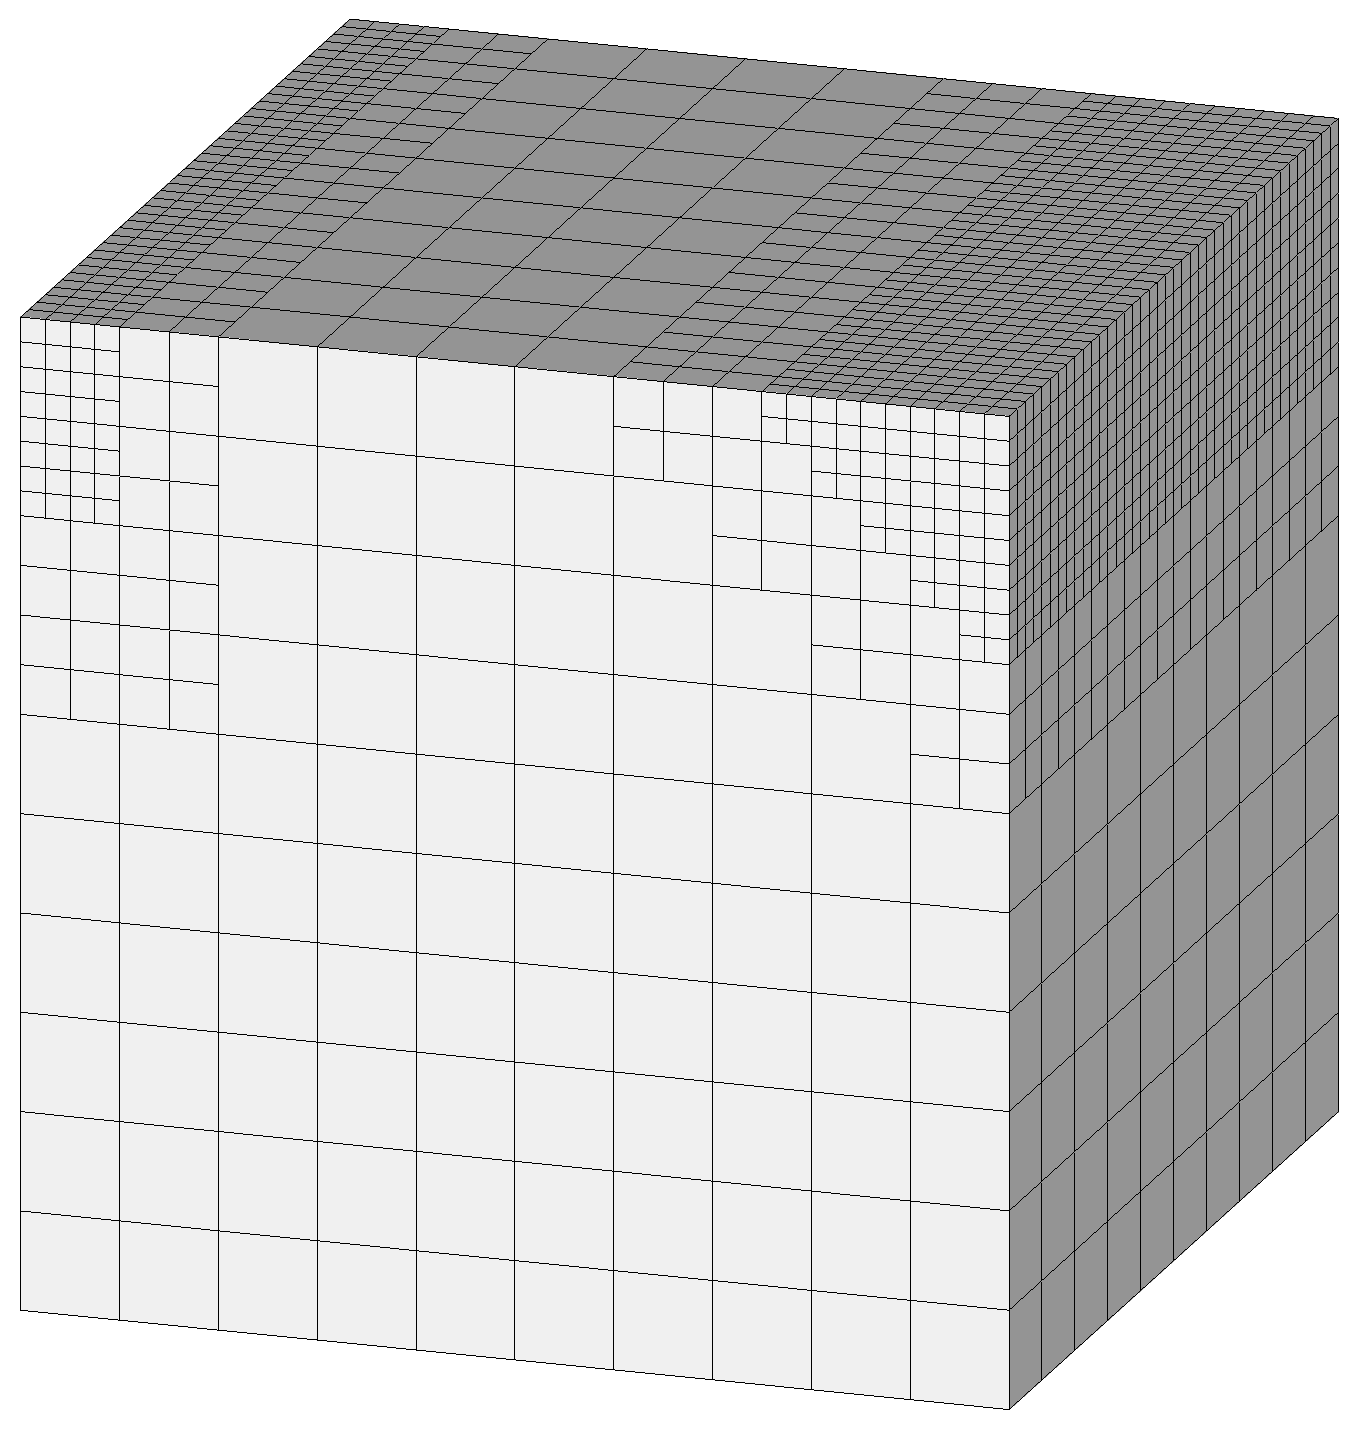
\includegraphics[scale=0.3]{cavfinal_p10_m30_p10.eps}
    \caption{Final grid for the cavity flow}
    \label{cavfinal_p10_m30_p10}
    \end{figure}
%%%%%%%%%%%%%%%%%%
    Few things have to be added at this point. Boundary markers     
    are only integers. On the surfaces where no boundary marker
    is specified, a default value 1 will be set. All the keywords for
    the {\tn Generator}, as well as for all the other principal
    programs are case {\em insensitive}. 
    
%----------------------------------------
    \paragraph{Example 2: A dune}
%----------------------------------------

    We continue with a slightly more complex problem domain
    shown in figure~(\ref{dune}). 
%%%%%%%%%%%%%%%%%%
    \begin{figure}
%%%%%%%%%%%%%%%%%%
    \centering
    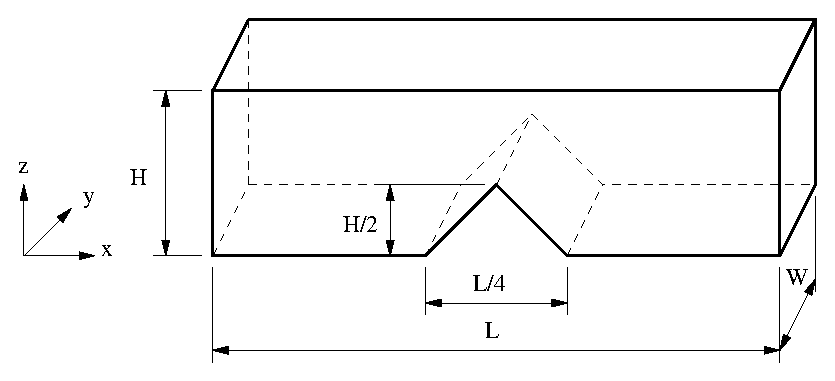
\includegraphics[scale=0.8]{dune.eps}
    \caption{Problem domain for the dune flow}
    \label{dune}
    \end{figure}
%%%%%%%%%%%%%%%%%%
    The purpose of this example
    is to illustrate the following:
    \begin{itemize}
    \item definition of a more complex, multi-block domain, 
    \item stretching of the grid lines toward the walls,  
    \item definition of the periodic boundary conditions.
    \end{itemize}
     
    To generate the grid for this test case, the domain first
    has to be decomposed into four blocks
      \footnote{This grid could have been generated with a
      single block, but we wanted to demonstrate the procedure
      for a multi block grid}. 
    One possible division and global point numbering is shown
    in figure~(\ref{duneblocks}). 
%%%%%%%%%%%%%%%%%%
    \begin{figure}
%%%%%%%%%%%%%%%%%%
    \centering
    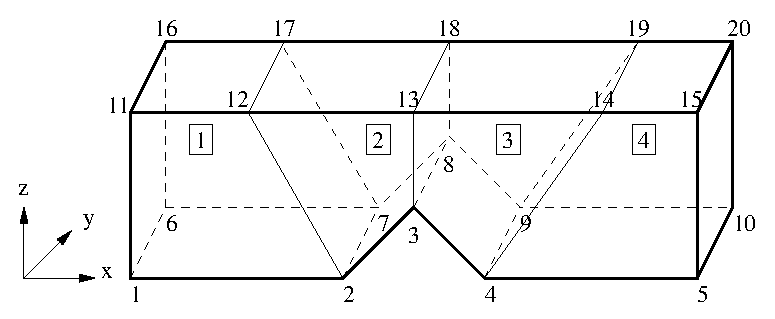
\includegraphics[scale=0.8]{duneblocks.eps}
    \caption{Global points for the dune}
    \label{duneblocks}
    \end{figure}
%%%%%%%%%%%%%%%%%%
    By setting $L=8$ and $H=2$, 
    we can define the
    points section of the domain as following:
    \small
    \begin{verbatim}
    #========#
    # Points #
    #--------#
    20

     1   0.0   0.0   0.0
     2   3.0   0.0   0.0
     3   4.0   0.0   1.0
     4   5.0   0.0   0.0
     5   8.0   0.0   0.0

     6   0.0   0.5   0.0
     7   3.0   0.5   0.0
     8   4.0   0.5   1.0
     9   5.0   0.5   0.0
    10   8.0   0.5   0.0

    11   0.0   0.0   2.0
    12   1.5   0.0   2.0
    13   4.0   0.0   2.0
    14   6.5   0.0   2.0
    15   8.0   0.0   2.0

    16   0.0   0.5   2.0
    17   1.5   0.5   2.0
    18   4.0   0.5   2.0
    19   6.5   0.5   2.0
    20   8.0   0.5   2.0 
    \end{verbatim}
    \normalsize
    To continue with block definition, we must decide on the
    local coordinates within each block. These can be defined
    in any sense, but we have adopted the one shown in 
    figure~(\ref{dunelocal}). 
%%%%%%%%%%%%%%%%%%
    \begin{figure}
%%%%%%%%%%%%%%%%%%
    \centering
    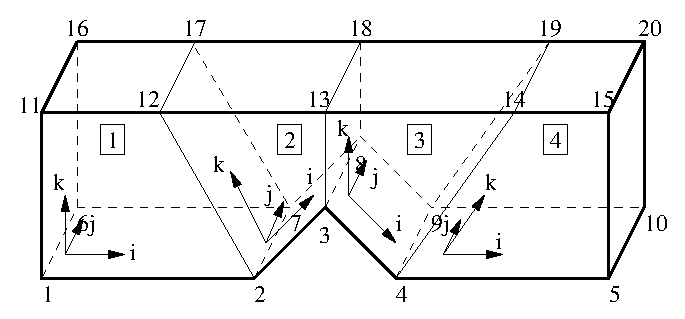
\includegraphics[scale=0.8]{dunelocal.eps}
    \caption{Local block coordinates for the dune}
    \label{dunelocal}
    \end{figure}
%%%%%%%%%%%%%%%%%%
    Following the local coordinate
    systems within each block, the block section of the domain
    file looks as follows:
    \small
    \begin{verbatim}
    #========#
    # Blocks #
    #--------#
     4
      1  20  5  30
        1.00  1.00  -0.9
        1  2  6  7 11 12 16 17
      2  16  5  30
        4.00  1.00  -0.9
        2  3  7  8 12 13 17 18
      3  16  5  30
        0.25  1.00  -0.9
        3  4  8  9 13 14 18 19
      4  20  5  30
        1.00  1.00  -0.9
        4  5  9 10 14 15 19  20         
    \end{verbatim}
    \normalsize
    For this example domain, the block weights are not all equal
    to one. For example, sub-domain 2 has weigth in i direction
    equal to 4.0. This tells the mesh generator to linearly stretch
    the cells towards the end in i direction by a factor of 4.
    The stretching factor is the ratio of the cell sizes in the
    beginning and the end of the local direction.  For all blocks
    the weigth in k direction is -0.9. Weights which are negative
    mean hyperbolic stretching. Further, weights in the range from
    -0.75 to -0.99 are for stretching toward both sides, whereas the
    weights from -0.25 to -0.75 are for hyperbolic stretching in 
    one direction only. All the weigth values and their meanings
    are summarised in table~(\ref{weigths}).
    \begin{table}
    \begin{tabular}{|l|l|}  \hline
      weigth:          & meaning: \\
       \hline 
      -0.999 to -0.751 & hyperbolical stretch in both directions \\
       \hline
      -0.749 to -0.501 & hyperbolical stretch to the origin of
                         local coordinate \\
       \hline
      -0.499 to -0.251 & hyperbolical stretch apart from origin 
                         of local coordinate \\
       \hline
      -0.249 to  0.000 & undefined \\
       \hline
       0.001 to  0.999 & linear stretching to the origin of 
                         local coordinate \\ 
       \hline
       1.001 to  1.000 & linear stretching apart from origin
                         of local coordinate \\ 
       \hline
    \end{tabular}
    \caption{Allowed weight values and their meaning}
    \label{weigths}
    \end{table}
    No lines and surfaces need explicit definition for this case,
    so the next two sections are as follows:
     \small
     \begin{verbatim}
     #---------#
     #  Lines  #
     #---------#
       0
     #------------#
     #  Surfaces  #
     #------------#
       0
     \end{verbatim}
     \normalsize
    For this test case we need only one boundary marker, and that
    is for solid walls in the top and in bottom of the domain. These 
    do not have to be specified, because by default they will be set to
    1. Therefore, the section for boundary conditions is:
    \small
    \begin{verbatim}
    #---------------------#
    # Boundary conditions #
    # (only the default)  #
    #---------------------#
      0
    \end{verbatim}
    \normalsize
    For this problem, periodic boundaries have to be specified 
    in both stream-wise ($x$)
    and span-wise ($y$) direction. To define the periodic boundaries
    we have to identify all pairs of block surfaces which have 
    connected and specify them by their points in domain file.
    For example, to connect the domain in stream-wise direction,
    we have to connect the surface \mbox{1-6-16-11} with the surface
    \mbox{5-10-20-15} (see figure~(\ref{duneblocks})). 
    To connect the domain in the span-wise 
    direction, we have to specify four more pairs of surfaces.
    The section for periodic boundary conditions in the domain
    file, looks as following:  
    \small
    \begin{verbatim}
    #=====================#
    # Periodic Boundaries #
    #---------------------#
      5
        1  1  6 16 11
           5 10 20 15
        2  1  2 12 11
           6  7 17 16
        3  2  3 13 12
           7  8 18 17
        4  3  4 14 13
           8  9 19 18
        5  4  5 15 11
           9 10 20 19  
    \end{verbatim}
    \normalsize
    For this example, we will not perform any local cell refinement
    so the next section is:
    \small
    \begin{verbatim}
    #============#
    # Refinement #
    #------------#
      0
    \end{verbatim}
    \normalsize
    The final grid for the flow around the cylinder is shown in
    figure~(\ref{dunefinal_p10_m30_p10}).
%%%%%%%%%%%%%%%%%%
    \begin{figure}
%%%%%%%%%%%%%%%%%%
    \centering
    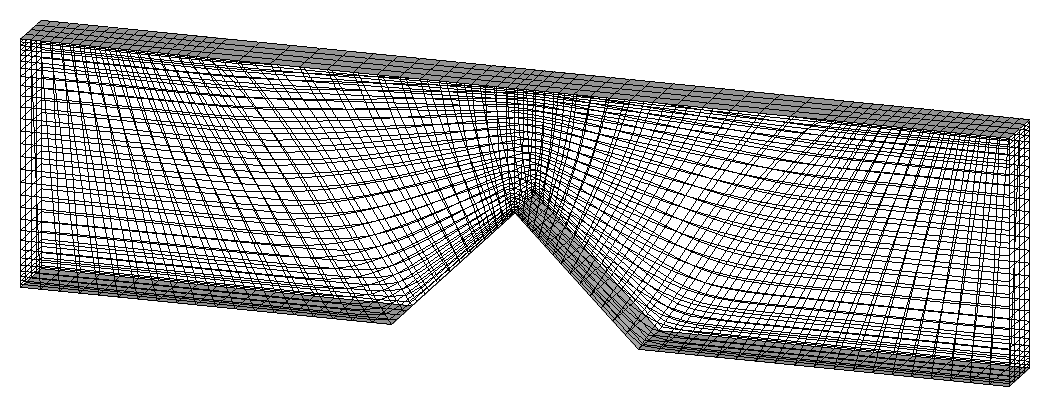
\includegraphics[scale=0.6]{dunefinal_p10_m30_p10.eps}
    \caption{Final grid for the dune flow}
    \label{dunefinal_p10_m30_p10}
    \end{figure}
%%%%%%%%%%%%%%%%%%

%----------------------------------------
    \paragraph{Example 3: A cylinder}
%----------------------------------------

    Next example is the domain for the calculation of the flow
    around the circular cylinder. It will demonstrate the following:
    \begin{itemize}
    \item definition of a more complex shape via the line section
          of the input file,
    \item refinement of an ellipsoidal region of the domain.
    \end{itemize}
    The problem domain is shown in figure~(\ref{cyl}).
%%%%%%%%%%%%%%%%%%
    \begin{figure}
%%%%%%%%%%%%%%%%%%
    \centering
    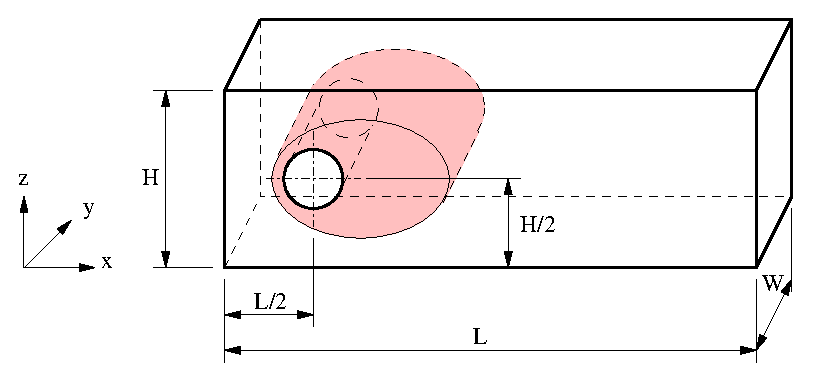
\includegraphics[scale=0.8]{cyl.eps}
    \caption{Problem domain for the flow around the cylinder}
    \label{cyl}
    \end{figure}
%%%%%%%%%%%%%%%%%%
    If we set the dimensions of the domain to: $L=9, H=3, W=3$,
    and if select the nodes as it is shown in figure~(\ref{cylpoints}),
%%%%%%%%%%%%%%%%%%
    \begin{figure}
%%%%%%%%%%%%%%%%%%
    \centering
    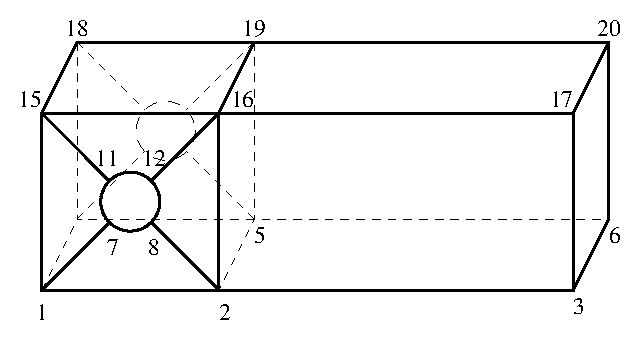
\includegraphics[scale=0.8]{cylpoints.eps}
    \caption{Problem domain for the flow around the cylinder 
             with specified point numbers. Some point numbers
             are omitted for the sake of clarity.}
    \label{cylpoints}
    \end{figure}
%%%%%%%%%%%%%%%%%%
    the point section of the input file might look as following:
    \small
    \begin{verbatim}
    %==========%
    %  Points  %
    %==========%
    20
    %-----------%
    %   Floor   %
    %-----------%
      1   0.0   0.0   0.0
      2   3.0   0.0   0.0
      3   9.0   0.0   0.0
      4   0.0   3.0   0.0
      5   3.0   3.0   0.0
      6   9.0   3.0   0.0
    %--------------%
    %   Cylinder   %
    %--------------%
      7   1.25   0.0   1.25
      8   1.75   0.0   1.25
      9   1.25   3.0   1.25
     10   1.75   3.0   1.25
     11   1.25   0.0   1.75
     12   1.75   0.0   1.75
     13   1.25   3.0   1.75
     14   1.75   3.0   1.75
    %----------%
    %   Roof   %
    %----------%
     15   0.0   0.0   3.0
     16   3.0   0.0   3.0
     17   9.0   0.0   3.0
     18   0.0   3.0   3.0
     19   3.0   3.0   3.0
     20   9.0   3.0   3.0
    \end{verbatim}
    \normalsize
    After the point section, we come to the line section, which
    is very important for this case, since the lines connecting
    the points around the cylinder (7-8-12-11 and 9-10-14-13)
    are not straight lines, but rather arcs. In the line section
    we must define 8 lines, i.e.\ 7-8, 8-12, 12-11, 11-8 (see
    figure~(\ref{cylpoints})) and 9-10, 10-14, 14-13, 13-9 
    (omitted in figure~(\ref{cylpoints})). So, the line section for
    this problem domain looks as:
    \small
    \begin{verbatim}
    %%%%%%%%%%%%%%%%%%%%
    %   line section   %
    %%%%%%%%%%%%%%%%%%%%
      8
    *---- line connecting points 8 and 12 
      1    8  12
        1    1.853554     .000000    1.146447
        2    1.880203     .000000    1.175276
        3    1.904509     .000000    1.206107
        4    1.926320     .000000    1.238751
        5    1.945503     .000000    1.273005
        6    1.961940     .000000    1.308658
        7    1.975528     .000000    1.345492
        8    1.986185     .000000    1.383277
        9    1.993844     .000000    1.421783
       10    1.998459     .000000    1.460770
       11    2.000000     .000000    1.500000
       12    1.998459     .000000    1.539230
       13    1.993844     .000000    1.578217
       14    1.986185     .000000    1.616723
       15    1.975528     .000000    1.654508
       16    1.961940     .000000    1.691342
       17    1.945503     .000000    1.726995
       18    1.926320     .000000    1.761249
       19    1.904508     .000000    1.793893
       20    1.880203     .000000    1.824724
       21    1.853553     .000000    1.853553
        .
        . 
    \end{verbatim}
    \normalsize
    We have shown here just one part of the line section, just
    the definition of the line 8-12. There
    are seven more lines defined in the same way. It is clear 
    from this example that {\tn Generator} is quite cumbersome
    to use. Theoretically it is capable of generating any domain,
    but in practice, that is far from an easy task. The user
    is therefore strongly advised to use some more sophisticated
    mesh generator instead of {\tn Generator}. The surface section
    for this case is empty, and the block section is formed in 
    the similar way to the block section of previous example (dune).
    and is not shown here in order to keep this user guide short.
    Boundary condition and periodic boundary sections are skipped
    from the same reason. In the refinement region, there is a
    feature which didn't occur in the previous examples, namely
    an ellipsoidal refinement region. It is described in the
    refinement section of the domain file in the following way:
    \small
    \begin{verbatim}
    %%%%%%%%%%%%%%%%%%
    %   refinement   %
    %%%%%%%%%%%%%%%%%%
     1
        1  1
           1   FILL ELIPSOID
               2.3  1.5  1.5  1.5  1000.0  1.0
    \end{verbatim}
    \normalsize
    The number of refinement levels is one (first line after
    the comments). In that level, only one region is refined
    (second line after the comment). The ellipsoidal region
    is specified by the keywords: {\tc FILL} and {\tc RECTANGLE}
    which is followed by six real numbers, first three of them
    specifying the $x$, $y$ and $z$ coordinates of ellipsoid, and the
    remaining three specifying the ellipsoid axes in $x$, $y$ and $z$
    directions respectively.  

    The final grid for the flow around the cylinder is shown in
    figure~(\ref{cylfinal_p10_m30_p10}).
%%%%%%%%%%%%%%%%%%
    \begin{figure}
%%%%%%%%%%%%%%%%%%
    \centering
    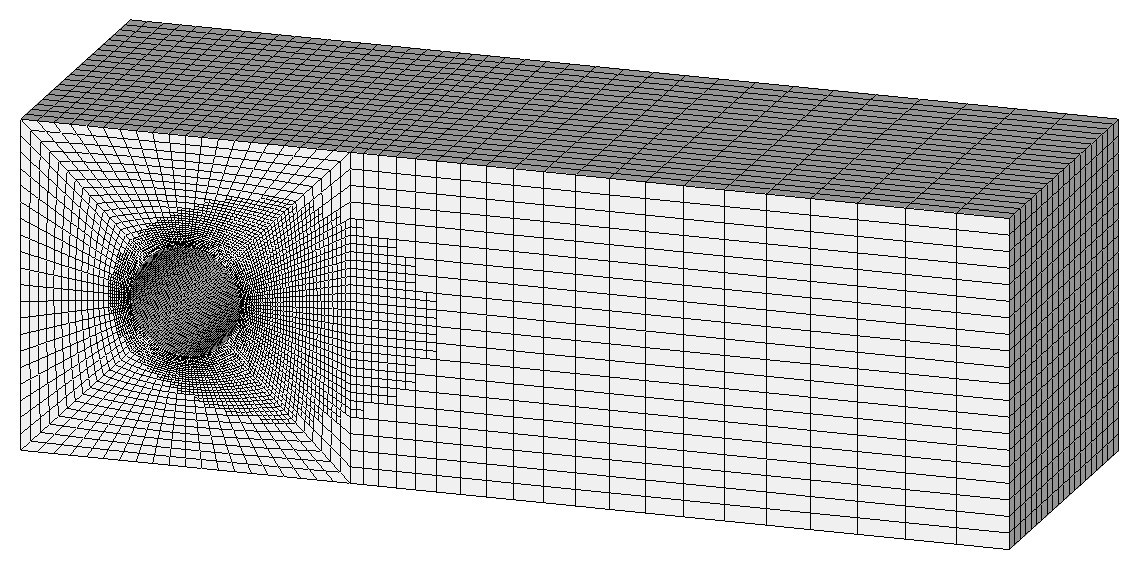
\includegraphics[scale=0.6]{cylfinal_p10_m30_p10.eps}
    \caption{Final grid for the flow around the cylinder}
    \label{cylfinal_p10_m30_p10}
    \end{figure}
%%%%%%%%%%%%%%%%%%

%================================================================
%
    \subsection{Using the {\tn Divisor}}
%
%================================================================

    {\tn Divisor} is used to divide the computational grid into
    an arbitrary number of sub-domains for subsequent parallel
    execution. If the user does not intend to run the {\tn Processor} 
    in parallel, he/she can skip this section.

    As an input, {\tn Divisor} requires the following input 
    files:
    \begin{itemize} 
      \item {\tc $<$NAME$>$.inp}
      \item {\tc $<$NAME$>$.cns} 
      \item {\tc $<$NAME$>$.geo} 
    \end{itemize}    
    As the output, it gives the following files:
    \begin{itemize} 
      \item {\tc $<$NAME$>$-0001.inp} -- {\tc $<$NAME$>$-$<$NSUB$>$.inp}
            AVS data files for each sub-domain. These are 
            needed just for visualisation of sub-domains and can
            safely be deleted to save the disk space.
      \item {\tc $<$NAME$>$-0001.gmv} -- {\tc $<$NAME$>$-$<$NSUB$>$.gmv}
            GMV data files for each sub-domain. These are 
            needed just for visualisation of sub-domains and can
            safely be deleted to save disk space.
      \item {\tc $<$NAME$>$-0001.cns} -- {\tc $<$NAME$>$-$<$NSUB$>$.cns}
            topology of the grid for each of the sub-domains. 
            Needed for parallel computations.
      \item {\tc $<$NAME$>$-0001.geo} -- {\tc $<$NAME$>$-$<$NSUB$>$.geo}
            geometrical quantities for each sub-domains. 
            Needed for parallel computations.
      \item {\tc $<$NAME$>$.inp} grid in AVS format, renumbered 
            for later visualisation of results.
      \item {\tc $<$NAME$>$.gmv} grid in GMV format, renumbered 
            for later visualisation of results.
      \item {\tc $<$NAME$>$-0001.ln.gmv} -- {\tc $<$NAME$>$-$<$NSUB$>$.ln.gmv}
            GMV data files for each sub-domain. These files were
            show the grid together with connectivity between 
            sub-domains. They were used during the debugging of
            {\tn Divisor} and are not needed for subsequent 
            calculations. The user can safely delete them to save
            some disk space. 
    \end{itemize}    

%-----------------------------------------------
    \subsubsection{Running the {\tn Divisor}}
%-----------------------------------------------
    
    The compilation of {\tn Divisor} is explained in section~(\ref{Com}).
    After running the {\tn Generator} it writes the logo on the screen
    and prompts the user with the
    following question:
    \small
    \begin{verbatim}
    Input problem name:
    \end{verbatim}
    \normalsize
    The same as it was with {\tn Generator}, the user has to enter
    the {\tc $<$NAME$>$} he used for mesh generation {\em without}
    extension. After it reads the necessary files, it will prompt
    the user with th question:
    \small
    \begin{verbatim}
    Number of sub-domains:
    \end{verbatim}
    \normalsize
    The user has to enter the desired number of sub-domains, which
    should be equal to the number of processors he/she would like
    to use. {\tn Divisor} is very quick and immediately writes
    more messages and then stops.

%================================================================
%
    \subsection{Using the {\tn Processor}}
%
%================================================================

    {\tn Processor} is the most important part of the {\tn T-Rex}
    package. It numerically solves the equations which govern the
    incompressible fluid flow with the control volume method. It 
    can be run in sequential or parallel mode. 

    If it is run in sequential mode, {\tn Processor} requires the 
    following input files:
    \begin{itemize} 
      \item {\tc $<$NAME$>$.cns} - created by {\tn Generator}
      \item {\tc $<$NAME$>$.geo} - created by {\tn Generator}
      \item {\tc $<$NAME$>$.b} - a file which specifies boundary
            conditions, 
      \item {\tc T-Rex.cmn} - a small script-like file with 
            instructions to generator. 
    \end{itemize}    
    If it is run in parallel, it requires the following files:
    \begin{itemize} 
      \item {\tc $<$NAME$>$-0001.cns} -- {\tc $<$NAME$>$-$<$NSUB$>$.cns} 
            - created by {\tn Divisor}
      \item {\tc $<$NAME$>$-0001.geo} -- {\tc $<$NAME$>$-$<$NSUB$>$.geo} 
            - created by {\tn Divisor}
      \item {\tc $<$NAME$>$.b} - a file which specifies boundary
            conditions, 
      \item {\tc T-Rex.cmn} - a small script-like file with 
            instructions to generator. 
    \end{itemize}    
    In both modes (sequential or parallel) it requires a single
    boundary condition file and a single command files. These files
    have to be created by the user, before running the 
    {\tn Processor}. 

%----------------------------------------------------------------
    \subsubsection{Running the {\tn Processor}}
%----------------------------------------------------------------

    The compilation of the {\tn Processor} is explained in
    section~(\ref{Com}).
    To run the {\tn Processor}, the user first have to go 
    to directory where all the necessary files are. Then he has
    to type the name of the {\tn Processor}'s executable name
    and it will open the {\tc T-Rex.cmn} command script and 
    start the execution. While running, it will print some 
    messages on the standard output which show the convergence history
    and some other details, like maximum CFL and Pe number,
    values of velocities and pressure at monitoring point,
    number of iterations for linear solver, etc. Before running
    the {\tn Processor}, the user has to be sure that he has created
    the boundary condition file and a {\tc T-Rex.cmn} script.
    
%----------------------------------------------------------------
    \subsubsection{The format of the boundary condition 
                   {\tc <NAME>.b} and the profile file}
%----------------------------------------------------------------

    This file is required by {\tn Processor}. It specifies the
    values of boundary conditions and fluid properties. It must
    have the same base name as the domain file {\tc <NAME>}
    and it must have the extension {\tc .b}
    It consists of two sections (and optional comments) and had to 
    be entered in the 
    following order:
    \begin{itemize}
    \item[1.] phisical properties of the fluid; dynamic viscosity and
              density 
    \item[2.] number of boundary markers and
              for each marker: it's id, type of boundary condition
              and the $u$, $v$ and $w$ value for velocities, {\em or}
              a keyword {\tc FILE} followed by the name of the file  
              where the velocity profile is given,
    \item comments - each line which begins with a character {\tc \#}
          or {\tc \%} is regarded as a comment line and skipped by the
          {\tn Processor}. Comment lines can appear anywhere in the
          input file.
    \end{itemize}
    The templated format of the boundary condition file is the following:
    \small
    \begin{alltt}
    1. <viscosity> <density>
    2. <num_markers>
       <marker_id 1> >type<  [INFLOW,OUTFLOW,WALL,SYMMETRY]  <u> <v> <w>
       [OR]
       <marker_id 1> >type<  [INFLOW,OUTFLOW,WALL,SYMMETRY]  FILE <file_name> 
       .
       .
       .
       <marker_id num_markers> >type<  [INFLOW,OUTFLOW,WALL,SYMMETRY]  <u> <v> <w>
       [OR]
       <marker_id num_markers> >type<  [INFLOW,OUTFLOW,WALL,SYMMETRY]  FILE <file_name> 
    \end{alltt}
    \normalsize 
%    As a type of boundary condition, user can enter on of the
%    following:
%    {tc INFLOW}
%    {\tc OUTFLOW}
%    {\tc WALL}
%    {\tc SYMMETRY}
%    which are case {\em insensitive}. The meaning of this 
%    keywords is quite clear and don't need further explanations. 
    For the values for velocity components, the user can enter 
    either three floating point numbers representing $u$, $v$
    and $w$ velocity components, or the keyword {\tc FILE}
    followed by the name of the file where the velocity profiles
    are stored. The format of the file with velocity profile is
    the following:
    \begin{itemize}
    \item[1.] Number of specified values in the profile
    \item[2.] coordinate direction of the profile; may be
              $x$, $y$ or $z$,
    \item[3.] List of coordinates and values
    \item comments - each line which begins with a character {\tc \#}
          or {\tc \%} is regarded as a comment line and skipped by the
          {\tn Processor}. Comment lines can appear anywhere in the
          input file.
    \end{itemize}
    \small
    \begin{alltt}
    The templated format of the profile file is the following:
    1. <num_values>
    2. >direction<  [X,Y,Z]
    3. <coordinate 1> <u> <v> <w>
       .
       .
       .
       <coordinate num_values> <u> <v> <w>
    \end{alltt}
    \normalsize
    \paragraph{Example: A cylinder}
    As an example, we give the boundary condition file which
    can be used for the calculation of the flow around the
    cylinder. The domain file ({\tc <NAME>.d}) for the flow
    around the cylinder was shown in section [].
    \small
    \begin{alltt}
    %-------------------------------------------------------------%
    % Boundary condition file for the flow around the cylinder    %
    %-------------------------------------------------------------%
    %-----------------------% 
    % viscosity and density %
    %-----------------------% 
     0.01  1.00
    %----------------------------% 
    % boundary condition markers %
    %----------------------------% 
      3
    %---------------------------------------------------%
    % this is the default boundary condition, allays 1 %
    %---------------------------------------------------%
      1         Wall         0.0      0.0   0.0
    %--------%
    % inflow %
    %--------%
      2         Inflow   File  parabolic-0-3.prof
    %---------%
    % outflow %
    %---------%
       3        Outflow  File  parabolic-0-3.prof
    \end{alltt}
    \normalsize
    This input file tells the processor to set the no slip 
    boundary conditions on the
    surfaces where marker is equal to 1,
    \footnote{remember that boundary marker 1 doesn't have to
              explicitly specified for {\tn Generator}, it will
              set marker to 1 at all the boundaries which are 
              not specified in the domain file}
    to set the inflow boundary conditions on the surfaces where
    the marker is equal to 2 and to set the outflow where marker
    is equal to 3. Further, it tells the {\tn Processor} to read
    the file {\tc parabolic-0-3.prof} to set the velocity components
    on the inflow and outflow boundaries. 
    The portion of the {\tc parabolic-0-3.prof} file is given
    bellow:
    \small
    \begin{alltt}
    #------------------#
    # Number of points #
    #------------------#
     200
    #-----------#
    # direction #
    #-----------#
     z
    #---------------------------------------#
    # coordinate U         V         W      #
    #---------------------------------------#
     .000000     .000000   .000000   .000000
     .010000     .019900   .000000   .000000
     .           .         .         .
     .           .         .         .
     .           .         .         .
     .990000     .999900   .000000   .000000
    1.000000    1.000000   .000000   .000000
    1.010000     .999900   .000000   .000000
     .           .         .         .
     .           .         .         .
     .           .         .         .

    1.990000     .019900   .000000   .000000
    2.000000     .000000   .000000   .000000
    \end{alltt}
    \normalsize
    There are no restriction on naming the profile files. Any
    name and extension allowed by the operating system
    may be used.

%----------------------------------------------------------------
    \subsubsection{The format of the command script {\tc T-Rex.cmn}} 
%----------------------------------------------------------------

    The command script {\tc T-Rex.cmn} contains the necessary 
    instruction for the {\tn Processor}. It has several sections,
    which must be entered in the following order:
    \begin{itemize}
    \item[1.]  problem name,
    \item[2.]  restart file name for loading or keyword skip
               to start the new simulation, 
    \item[3.]  number of time steps user wants to perform,
    \item[4.]  time step at which user wants to start to gather
               the statistics,
    \item[5.]  coordinates of the monitoring point,
    \item[6.]  coordinates of the monitoring plane,
    \item[7.]  type of simulation; DNS or LES and for LES the
               value of the Smagorinsky constant,
    \item[8.]  type of the problem to be solved,
    \item[9.]  algorithm for linking velocities and pressure;
               can be either fractional step or SIMPLE; if
               SIMPLE, then also the under-relaxation factors
               for velocity and pressure,
    \item[10.] time stepping schemes for different parts of the
               discretised system of equations,
    \item[11.] upwind blending, yes or no, and if yes, then the
               amount of central differencing used,
    \item[12.] tolerance for linear solvers for velocity and
               pressure; for SIMPLE also the tolerance for
               outer iterations,
    \item[13.] time step
    \item[14.] pressure drop ($b$ from equation~(\ref{pressure}),
    \item[15.] desired mass flux for flows in periodic domains,
    \item[16.] restart file name for saving,
    \item[17.] file format for saving the results; the results
               can be saved in either GMV or AVS format,
    \item[18.] result file name 
    \item[19.] unused; a keyword skip
    \item[20.] Number of time step; the same as under 3.
    \item[21.] if under 21.\ user has typed nonzero, the same as
               under 4.\, etc.         
    \item comments - each line which begins with a character {\tc \#}
          or {\tc \%} is regarded as a comment line and skipped by the
          {\tn Processor}. Comment lines can appear anywhere in the
          input file.
    \end{itemize}
    The exact format of the {\tc T-Rex.cmn} command script now
    follows:
    \small
    \begin{alltt}
     1. <NAME>
     2. <restart_file_name> [OR] skip
     3. <num_time_steps>
     4. <start_statistics>
     5. <x_point> <y_point> <z_point>
     6. <x_plane> <y_plane> <z_plane>
     7. >type_simulation< [DNS,LES]
        <Cs> 
     8. >type_problem<   [CHANNEL,OTHER]
     9. >type_algorithm< [FRACTION,SIMPLE]
        <urf_u>
        <urf_p>
    10. >time_stepping_convection<     [AB,CN,FI]
        >time_stepping_diffusion<      [AB,CN,FI]
        >time_stepping_cross_difusion< [AB,CN,FI]
    11. >upwind_blending<              [YES,NO]
        <blend_coeff>
    12. <eps_uvw>
        <eps_p>
        <eps_simple>
    13. <delta_t>
    14. <p_drop>
    15. <flux_o>
    16. <restart_file_name> [OR] SKIP 
    17. >result_format< [AVS,GMV]
    18. <result_name>
    19. SKIP 
    20. <num_time_steps>
    21. <start_statistics>
        .
        .
        .
    \end{alltt}
    \normalsize

%================================================================
%
    \newpage
    \section{Visualisation of results}
%
%================================================================

    As it was said above, the results can be visualised either
    by the AVS or by the GMV package. In both cases, one needs
    the files created by the {\tn Generator} and {\tn Processor}.
    In the file created by generator ({\tc <NAME>.inp} for AVS and
    {\tc <NAME>.gmv for GMV}), a computational grid is 
    defined, whereas in the file created by the processor 
    ({\tc <NAME>.r.inp} for AVS or {\tc <NAME>.r.gmv} for GMV) the
    results are stored. This files have to be connected if one
    wants to visualise the results. Currently, it is done by the
    UNIX {\tc cat} command as following:
    \begin{alltt}
    cat <NAME>.inp <NAME>.r.inp > <RESULTNAME>.inp
    \end{alltt}
    to create the input file for AVS, or by:
    \begin{alltt}
    cat <NAME>.gmv <NAME>.r.gmv > <RESULTNAME>.gmv
    \end{alltt}
    Unfortunately, this is not all. The files created in such a way
    are not complete yet. 
    For AVS, one has to edit the result file ({\tc <RESULTNAME>.inp})
    and change the first line which currently looks as:
    \begin{alltt}
    <num_nodes> <num_cells> <num_ndata> <num_cdata> <num_mdata>
    \end{alltt}
    to: 
    \begin{alltt}
    <num_nodes> <num_cells>    0    14     0 
    \end{alltt}
    and save the file. Further details on AVS data format are in 
    the section (\ref{avsformat}).

    For GMV, however, one has to edit the result file 
    ({\tc <RESULTNAME>.gmv}) and find the first occurrence of the
    line which contains the keyword {\tc endgmv}. This line has to
    be erased, and file saved. The details of the GMV data format 
    are in the section (\ref{gmvformat}).  

    If the computation was run in parallel, instead of one result
    file name ({\tc <NAME>.r.gmv}) the user gets one result file for each
    processor, ({\tc <NAME>-0001.r.gmv} -- {\tc <NAME>-<NSUB>.r.gmv}).
    Before making the changes described above, the user has to
    connect the result files into a single file. 
    {\tn Connect} utility is used for that purpose. To compile
    it, the user has to go to {\tc T-Rex/Test}
    directory and run:
    \begin{alltt}
    gmake connect
    \end{alltt}
    The executable named {\tc CON} will be created in the same
    directory. Running the {\tc CON} without any arguments will
    print the information about it's usage.  


%================================================================
%
    \newpage
    \section{Using the {\tn F2html}}
%
%================================================================

    In order to use {\tn F2html}, you have to create an ASCII
    file with list of all sources and include files you want to 
    convert into html format. You have to create this file in
    the directory you want the html files to be created. We 
    suggest to choose {\tc T-Rex/DOC/html} which already
    exists after unpacking the {\tn T-Rex} package. To create
    the list of source files, you type the following:
      \footnote{a small shell script called {\tc list.sh}
      can do that job for you}
    \small
    \begin{alltt}
    ls -1 ../T-Rex/Gen/*.f > list.dat
    ls -1 ../T-Rex/Gen/*.h >> list.dat
    ls -1 ../T-Rex/Div/*.f >> list.dat
    ls -1 ../T-Rex/Div/*.h >> list.dat
    ls -1 ../T-Rex/Pro/*.f >> list.dat
    ls -1 ../T-Rex/Pro/*.h >> list.dat
    ls -1 ../T-Rex/Par/*.f >> list.dat
    ls -1 ../T-Rex/Par/*.h >> list.dat
    ls -1 ../T-Rex/Lib/*.f >> list.dat
    ls -1 ../T-Rex/Lib/*.h >> list.dat
    \end{alltt}
    \normalsize
    To create the list of all source needed for compilation of
    the parallel version of {\tn T-Rex}. 

    When the list of sources is created, you can start the
    {\tn F2html}. When it starts, it will prompt you with 
    the following question:
    \small
    \begin{alltt}
    Input the project name:
    \end{alltt}
    \normalsize
    you have to type the name of the project as you want it
    to appear on the html pages. The best one is probably
    {\tc T-Rex}. When you enter the desired name, it will ask
    you for the file with the list of source:
    \small
    \begin{alltt}
    Input the file name with list of sources:
    \end{alltt}
    \normalsize
    You have to reply with the name of the file which has the
    list of all sources. If you have followed the suggestions
    above, it is {\tc list.dat}
    Then it starts the conversion process. You can notice that it
    is running, because it writes many messages on the screen.
    After a minute or two, a complete package in html format
    resides in the current directory. To start viewing it,
    run some web browser (netscape, for example) with the 
    command:
    \small
    \begin{alltt}
    netscape index.html
    \end{alltt}
    \normalsize
    It will open the browser window with the front page of the
    {\tn T-Rex} package. How it looks on our system is shown in
    figure~(\ref{browser1}). Note that there are two frames
    in the browser: the right for the source listings
    and the left one for some useful diagrams.
    If you click on the program name
    it will bring the listing of the main procedure to the
    right frame. An example is shown in figure~(\ref{browser2}).
    Note that there are four link after each function/subroutine
    name:
    \begin{itemize}
    \item it's own name: brings the flow diagram in the left
          frame
    \item arrow left: brings the {\em call by} view in the left
          frame
    \item arrow right: brings the {\em invocation} view in the left
          frame
    \item arrow up: brings the main page back to the right frame.
    \end{itemize}

    We strongly believe that sources in the linked html format
    are the best way to understand how the {\tn T-Rex} package
    works. And yet, it takes less then a minute to (re)create
    new html pages if something changes in the code. However,
    since we have developed {\tn F2html} just for our local use,
    we cannot that it will work with any other Fortran program
    but {\tn T-Rex}. 

%%%%%%%%%%%%%%%%%%
    \begin{figure}
%%%%%%%%%%%%%%%%%%
    \centering
    \includegraphics[scale=0.3]{browser1.eps}
    \caption{F2html front screen}
    \label{browser1}
    \end{figure}
%%%%%%%%%%%%%%%%%%

%%%%%%%%%%%%%%%%%%
    \begin{figure}
%%%%%%%%%%%%%%%%%%
    \centering
    \includegraphics[scale=0.3]{browser2.eps}
    \caption{F2html in action}
    \label{browser2}
    \end{figure}
%%%%%%%%%%%%%%%%%%


%================================================================
%
    \clearpage
    \newpage
    \section{Numerical method}
%
%================================================================

%================================================================
    \subsection{Main features}
%================================================================

    \begin{itemize}
    \item Second order finite volume method on unstructured grid
    \item Grids of any topology and any cell type are supported.
          Hexahedronal, tetrahedronal girds, hybrid grids.  
    \item Local grid refinement by cell splitting possible. 
    \item Different time integrations schemes: 
    \begin{itemize}
       \item fully implicit SIMPLE
       \item semi-implicit fractional step method  
       \item explicit Euler
       \item Adams Bashforth
    \end{itemize}
    \item Diffusive terms discretised in a least-squares sense
    \item Convective terms discretised with central differences,
          may be blended with upwind. 
    \item Linear system for pressure solved by a PCCG method
          and linear system for velocities by a PCBICG method.  
    \end{itemize}

    \begin{figure}[h]
    \centering
    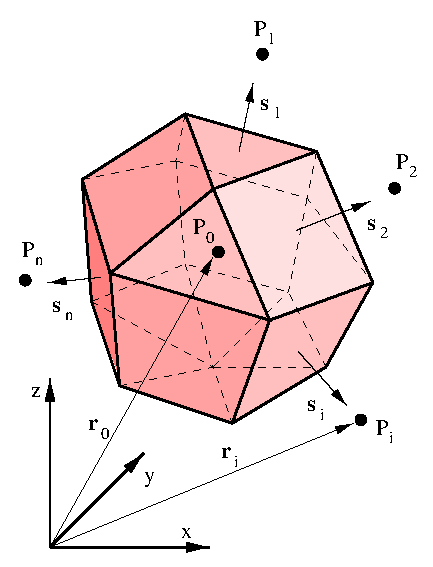
\includegraphics[scale=0.8]{molecule.eps}
    \caption{Computational cell}
    \end{figure}

%================================================================
    \subsection{Spatial discretisation}
%================================================================

    In present approach, a linear spatial distribution is assumed
    inside the control volume:
    \begin{equation}  
    \phi({\bf r},t) = 
      \phi_0(t) + 
      {\bf g}_0 ({\bf r} - {\bf r}_0)
      \label{distribution} 
    \end{equation}
    where $\phi$ is dependent variable ${\bf g}$ stands for the
    gradients of dependent variable in the control volume and
    ${\bf r}$ is the position vector.  The gradient vector ${\bf g}$
    is calculated by ensuring that equation \ref{distribution}
    is satisfied for nearest neighbours of $P_0$, i.e.\ by solving
    the following set of equations:
    \begin{equation}  
    {\bf d}_i \cdot {\bf g}_0 = \phi_i - {\phi}_0
    \hspace{1cm} 
    (i=1,\dots,n)
    \label{grad1} 
    \end{equation}
    where ${\bf d}_i = {\bf r}_i - {\bf r}_0$ is the distance
    vector between the centre of the control volume $P_0$ and
    its neighbour $P_i$ and $n$ is the number of neighbours.
    If the grid consists of tetrahedron only, the equation 
    (\ref{grad1}) is sufficient to find the gradient vector ${\bf g}$ 
    If the number of neighbours is greater then three, equation
    (\ref{grad1}) represents an overdetermined set of equations.
    In such a case, a {\em least square method} is used to find
    the components of gradient vector ${\bf g}$. The application 
    of the least square method results in the following system
    of equations:
    \begin{equation} 
    {\bf D} \cdot {{\bf g}_P}_0 = {\bf f}
    \label{grad2} 
    \end{equation}
    where 
    \begin{equation}  
    {\bf D} = \sum_{i=1}^{n} {\bf d}_i^T{\bf d}
    \hspace{0.5cm}
    and 
    \hspace{0.5cm} 
    {\bf f} = \sum_{i=1}^{n} {\bf d}_i^T{\phi_i - \phi_0}
    \label{grad3} 
    \end{equation}
    It is important to note ${\bf D}$ is a symmetric $3 \times 3$
    matrix whose coefficients depend on the cell centre coordinates
    only. Therefore, for a single grid, it is sufficient to calculate
    it only once before the calculations. However, this matrix is
    not the same for velocities and pressure due to different boundary
    conditions. This means that two
    gradient matrices have to be stored, one for velocity components
    and one for pressure. That might lead to excessive memory 
    consumption, which is particularly important on distributed 
    memory parallel computers, where each processor has only 
    limited amount of memory. Having that in mind, we recalculate
    the gradient matrix before each calculation of gradients of
    velocity and pressure. 
        


    Least squares method for calculation of $ (grad \phi)_0 $  
    Cell face value:
    \begin{equation}
    \phi_j = \frac{1}{2} [ (\phi_0 + \phi_i) 
           +   {\bf g}_0 ({\bf r}_j - {\bf r}_0) +
               {\bf g}_i ({\bf r}_j - {\bf r}_i) ]
    \label{cellface}
    \end{equation}

%================================================================
    \subsection{Convection}
%================================================================

    The convective flux through the cell face $j$ is approximated
    as:
    \begin{equation}
      C_j = \int_{S_j} \rho \phi {\bf u} \cdot {\bf n} \approx
         F_j \cdot \phi_j   
    \end{equation}
    where $\phi_j$ is the cell face value, and is calculated
    from the following equation: 
    \begin{equation}
    \phi_j^{cd} = \frac{1}{2} [ (\phi_0 + \phi_i) 
               +   {\bf g}_0 ({\bf r}_j - {\bf r}_0) +
                   {\bf g}_i ({\bf r}_j - {\bf r}_i) ]
    \label{cellfaceCD}
    \end{equation}
    Such an approximation of cell face
    value is the second order accurate central differencing.
    But, when calculation the flows at higher Reynolds numbers,
    it can lead to numerical instabilities. The well known
    cure for that problem is the upwind differencing for 
    convection, which is: 
    \begin{equation}
    \phi_j^{up} = \left\{
                  \begin{array}{ll}
                  \phi_0 & \mbox{if $F_j > 0$} \\
                  \phi_i & \mbox{if $F_j < 0$}
                  \end{array}
                  \right. 
    \end{equation}
    This reduces the order of the scheme to first order, which 
    should be avoided for LES of turbulence. To combine the
    stability of the upwind scheme, and the second order accuracy
    of the central scheme, we use the {\em deffered correction}
    approach, which may be summarised as follows:
    \begin{equation}
    \phi_j = \left\{
             \begin{array}{ll}
             \phi_0^{up} + \gamma (\phi_i^{cd}-\phi_0^{up}) & \mbox{if $F_j > 0$} \\
             \phi_i^{up} + \gamma (\phi_0^{cd}-\phi_i^{up}) & \mbox{if $F_j < 0$}
             \end{array}
             \right. 
    \end{equation}
    where $\gamma$ is factor between 0 and 1. The closer is
    $\gamma$ to 1, the closer we are to the central differencing.

%================================================================
    \subsection{Diffusion}
%================================================================

    Diffusion flux through cell face $j$ is approximated as
    \begin{equation}
      D_j = - \int_{S_j} \Gamma_\phi \nabla \phi {\bf n} d {\bf S}
             \approx
             (\Gamma_{\phi} {\nabla \phi})_j^\star \cdot {\bf S}_j  
    \end{equation}
    Gradient on the cell face is discretised by a {\em deffered
    correction} approach:
    \begin{equation}
      ({\nabla \phi})_j^\star = 
      \overline{ ({\nabla \phi}) }_j  + 
      [
          \frac{ \phi_j - \phi_0}  
               {| {\bf d}_j |} 
        - \frac{ \overline{ ({\nabla \phi}) }_j \cdot {\bf d}_j } 
               {| {\bf d}_j |} 
      ] 
      {\bf n}_j
    \end{equation}
    Where the over bar means the arithmetic average between cell
    centres $P_0$ and $P_i$. If we insert the equation for the
    gradient on the cell face into the equation for diffusive
    flux, and knowing that ${\bf n}_j ={\bf S}_j / |{\bf S}_j|$,
    we get the following equation for the diffusive flux: 
    \begin{equation}
      D_j = 
      \Gamma_j (\phi_j - \phi_0) \frac{|{\bf S}_j|}{|{\bf d}_j|}
      +
      \Gamma_j 
      \overline{ ({\nabla \phi}) }_j {\bf S}_j 
      -
      \Gamma_j 
      \overline{ ({\nabla \phi}) }_j  
      {{\bf d}_j} \frac{|{\bf S}_j|}{|{\bf d}_j|}
    \end{equation}
 
%================================================================
%
    \newpage
    \section{Turbulence model}
%
%================================================================

%----------------------------------------------------------------
    \subsection{Smagorinsky model}
%----------------------------------------------------------------

    The equations which describe the incompressible fluid flow
    are the continuity equation:
    \begin{equation}
    \frac{\p u_i}{\p x_i}=0
    \label{cont}
    \end{equation}
    and the Navier-Stokes equation:
    \begin{equation}
    \frac{\p u_i}{\p t}+
    \frac{\p u_i u_j}{\p x_j}=
    \frac{1}{\rho}\frac{\p p}{\p x_i} + 
    \frac{\p}{\p x_i}(\nu (\frac{\p u_i}{\p x_j}+\frac{\p u_i}{\p x_j}))
    \label{navsto}
    \end{equation}
    Equations (\ref{cont}) and (\ref{navsto}) are capable of describing
    both laminar and turbulent flows. For laminar flows, this does not
    poses any particular problem. But, in order to use the equations 
    (\ref{cont}) and (\ref{navsto}) for the solution of turbulent flows
    the numerical grid has to be fine enough to capture all the scales
    of motion and the time step should be small enough to resolve the
    life time off all the eddies in the flow. This requirement puts very
    high demands on computer hardware, which, at the present time is 
    not capable to match those requirements. The solution of turbulent
    flows is therefore seeked via the turbulence model. The main idea
    of LES of turbulence is to solve the equations on the grid which 
    is coarser then small eddies in the flow and account for them through
    the sub-grid scale model. In LES framework, this solution on the
    coarse mesh is called {\em filtering}. If the governing equations
    are solved with the control volume method, implicit filtering is 
    almost invariantly applied, which means that the computational
    cells are supposed to act as spatial filters on the governing
    equations. The filtered continuity and Navier-Stokes equations
    are:
    \begin{equation}
    \frac{\p \ol{u}_i}{\p x_i}=0
    \label{fcont}
    \end{equation}
    \begin{equation}
    \frac{\p \ol{u}_i}{\p t}+
    \frac{\p \ol{u_i u_j}}{\p x_j}=
    \frac{1}{\rho}\frac{\p p}{\p x_i} + 
    \frac{\p}{\p x_i}(\nu (\frac{\p \ol{u}_i}{\p x_j}+\frac{\p \ol{u}_i}{\p x_j}))
    -\frac{\tau_{ij}}{x_j}
    \label{fnavsto}
    \end{equation}
    where $\ol{u}$ is the filtered velocity, which is the difference
    between the real velocity and the sub grid scale velocity:
    \begin{equation}
    \ol{u}_i = u_i - u'_i
    \end{equation}
    The term $\tau_{ij}$ accounts for the difference between the
    non-filtered and filtered and non-linear terms:
    \begin{equation}
    \ol{u_i u_j} = \ol{\ol{u}_i \ol{u}_j}
                 \underbrace{
                 + \ol{\ol{u}_i u'_j} 
                 + \ol{u'_i \ol{u}_j} 
                 + \ol{u'_i u'_j}
                 }_{\tau_{ij}} 
    \end{equation} 
    The main idea (hope) of LES approach is that this difference
    expressed with $\tau_{ij}$ is rather small and tends to be 
    more universal from one flow case to another. Another feature
    of this term is that it diminishes as the grid is refined.
    Since $\tau_{ij}$ cannot be computed from the large scale
    values, a model has to be introduced to compute it. If a
    Smagorinsky model is used, this, sub-grid scale stresses are
    modelled as being proportional to the strain in the large
    scale field:
    \begin{equation}
    \tau_{ij} = -2 \nu_t \ol{S}_{ij} 
              = -\nu_t (\frac{\p \ol{u}_i}{\p x_j}+\frac{\p \ol{u}_i}{\p x_j})  
    \label{tau}
    \end{equation} 
    where $\nu_t$, eddy viscosity is represented as:
    \begin{equation}
    \nu_t = (C_S \Delta)^2 |\ol{S}|
    \end{equation} 
    In the above equation, $\Delta$ is the filter width and in
    our approach (program) it is computed as:
    \begin{equation}
    \Delta = min(V^{\frac{1}{3}}, \delta)
    \end{equation}
    where $V$ is the volume of the computational cell, and $\delta$
    is the distance from the cell centre to the nearest wall. By
    calculating the filter width in such a way, we damp the 
    eddy viscosity in the near-wall regions, which is important
    for wall-bounded flows. 
    The strain rate is computed as:
    \begin{equation}
    |\ol{S}| = (\ol{S}_{ij} \ol{S}_{ij})^{\frac{1}{2}} 
             = (S_{11}+S_{22}+S_{33}
                + 2 S_{12} S_{21}
                + 2 S_{13} S_{31}
                + 2 S_{23} S_{32} ) ^ {\frac{1}{2}}
    \end{equation}
    If the equation (\ref{tau}) is introduced into~(\ref{fnavsto}),
    we get the following form of the equations to be solved: 
    \begin{equation}
    \frac{\p \ol{u}_i}{\p t}+
    \frac{\p \ol{u_i u_j}}{\p x_j}=
    \frac{1}{\rho}\frac{\p p}{\p x_i} + 
    \frac{\p}{\p x_i}(\nu_{\mathit{eff}} (\frac{\p \ol{u}_i}{\p x_j}+\frac{\p \ol{u}_i}{\p x_j}))
    \label{fnavsto2}
    \end{equation}
    where $\nu_{\mathit{eff}}$ is the effective viscosity obtained 
    from:
    \begin{equation}
    \nu_{\mathit{eff}} = \nu + \nu_t
    \label{eddy}
    \end{equation}
    It is clear from equation~(\ref{fnavsto2}) that the sub-grid
    scale terms act as a drain of energy, which is quite normal
    for an eddy viscosity model, such as the Smagorinsky.  

    Practically, the implementation of the Smagorinsky model 
    consists of calculation of eddy viscosity according to
    equation~(\ref{eddy}) and adding it to the laminar viscosity.
    The calculation of eddy viscosity is performed in {\tc SGS.f}
    subroutine, and the discretisation of filtered Navier-Stokes
    equations is performed in {\tc NewUVW.f} subroutine. That is
    very simple when compared to the implementation of any RANS
    model, but we have to bear in mind that the main idea of LES
    is to use simpler turbulence models and more computational
    power.   

%----------------------------------------------------------------
    \subsection{Wall function}
%----------------------------------------------------------------

    The near wall layer should be either fully resolved, or the
    wall function should be used to bridge the laminar and the
    buffer region of the flow. Experience says that the wall 
    function should be used only when the first computational 
    points falls beyond $y^+=30$. 
      \footnote{where $u^+=u/u_{\tau}$  
                and  $u_{tau}=(\tau_w/ \rho)^{1/2}$}
    In our code, the Werner and Wengle
    wall function is employed. It assumes the linear profile 
    $u^+=y^+$
    from $y^+=0$ to $y^+=11.81$ and is continued by the power
    law of the form: $u^+=A(y^+)^B$ (with $A=8.3$ and $B=1/7$).

    Practically, we first calculate the $u_{\tau}$ in the cell closest
    to the wall from the power law:
    \begin{equation}
      u_{\tau} = \left[ 
                    \frac{u_t}{A} 
                       \left( \frac{\nu}{\delta}
                       \right)^B
                 \right]^{\frac{1}{1+B}}
    \end{equation}
    where $u_t$ is a velocity component tangential to the wall
    and $\delta$ is the closest distance to the wall.
    Then we calculate $y^+$ from the following equation:
    \begin{equation}
      y^+ = \frac{ \delta u_{\tau} }{ \nu }
    \end{equation}
    When $u_{\tau}$ and $y^+$ are calculated, we set the effective 
    viscosity
    in the cell near to the wall according to:
    \begin{eqnarray}
      \mu_{\mathit{eff}}=\frac{ \rho \delta u_{\tau}^2 }{ |u_t| } 
                \; \; \; \; \mbox{if} \; \; \; \; y^+ > 11.81 \\
      \mu_{\mathit{eff}}=\mu \;\;\;\;\;\; otherwise
    \end{eqnarray}

         
%================================================================
%
    \newpage
    \section{Auxiliary computational details}
%
%================================================================

%----------------------------------------------------------------
    \subsection{Storage of the matrices arising from the
                discretisation on locally refined grids}
%----------------------------------------------------------------

    Since we have developed an {\em unstructured} FV solver, stencil
    size can range from cell to cell. Nevertheless, the linear system
    arising after the discretisation of the governing equations is
    sparse. Unfortunately, although there are many possible ways for
    storing sparse matrices, none of them represents any kind of
    standard. Therefore we have decided to store
    the matrix in a slightly modified {\em sparse column format} used
    on the Cray UNICOS systems. 
    The modified sparse column format is described bellow.
    Suppose that $A$ is a $5 \times 5$ matrix defined as follows:

    \begin{equation}
     A=
     \left [
     \begin {array}{r} 
        50  \\   0  \\   0  \\  33  \\   0
     \end {array}
     \begin {array}{r} 
         0  \\  60  \\  45  \\   0  \\  37
     \end {array}
     \begin {array}{r} 
          0  \\  46  \\  65  \\  47  \\   0 
     \end {array}
     \begin {array}{r} 
         34  \\   0  \\  49  \\  66  \\  0
     \end {array}
     \begin {array}{r} 
          0  \\  38  \\   0  \\   0  \\  70
     \end {array}
     \right ]
                                \label{A}
    \end{equation}
    The matrix $A$ is stored in one array ({\tc A\_val}), by 
    inserting non--zero
    entries, column by column. Two additional integer arrays
    are also needed by the original sparse column format,
    {\tc Arow} which specifies the row number of each entry
    in the vector {\tc Aval}, and {\tc Acol} which points to
    a beginning of the each column in arrays {\tc A\_val} and
    {\tc Arow}. We have also added the {\tc Adia} array
    which points to the diagonal entries of the system matrix.
    This additional array significantly simplifies the coding
    and slightly improves the performance of the Krylov
    subspace iterative linear solvers.
    \small \begin{verbatim}
      REAL    :: Aval(NONZER)
      INTEGER :: Arow(NONZER)
      INTEGER :: Acol(NC+1)
      INTEGER :: Adia(NC)    ! <--- points to diagonal entries 

      DATA A_val  /50,33,60,45,37,46,65,47,34,49,66,38,70 /
      DATA A_row  / 1, 4, 2, 3, 5, 2, 3, 4, 1, 3, 4, 2, 5 /
      DATA A_col  / 1, 3, 6, 9,12,14 /
      DATA Adia   / 1, 3, 7,11,13 / 
    \end{verbatim} \normalsize
    \vspace{-0.2in}
    The fragment of the Fortran~90 code which stores the matrix
    $A$ from (\ref{A}) in a modified column sparse format is
    shown above. \texttt{NONZER} is a total number of non--zero
    entries in the system matrix and is the most conveniently
    calculated during the grid generation process.

%----------------------------------------------------------------
    \subsection{Keeping the constant mass flux for 
                unsteady, spatially periodic flows}
%----------------------------------------------------------------

    When solving the fluid flow in the periodic geometry, one
    faces the problem of keeping the mass flux constant. The
    usual practice is to solve the velocities with periodic
    boundary conditions and to decompose the pressure into
    periodic and linear part:
    \begin{equation}
    P(x,y,z,t) = \underbrace{p(x,y,z,t)}_{\mbox{periodic part}} 
               + \underbrace{b(t) \cdot x}_{\mbox{linear part}}
    \label{pressure}
    \end{equation}
    For the solution of periodic part of the pressure, a
    usual periodic boundary conditions are solved, and the
    linear part, when inserted into Navier-Stokes equations,
    act as a driving force. The periodic part of the 
    pressure keeps the velocity field divergence free,
    whereas the linear part (pressure drop) determines the flow rate through
    the domain. If the geometry of the flow is simple, (like
    a channel or a pipe) one usually prescribes the pressure
    drop to be constant it time, which gives almost 
    constant flow rate. However, such a practice, when 
    applied in complex geometries, can result in relatively
    big variations of the flow rate which contaminate the LES
    results, since these variations are interpreted as additional
    stream-wise Reynolds stresses. To avoid this effect, we have
    tried several practices, but none of them
    was fully satisfactory. Very recently, we have implemented
    a new practice which seems to work well with all the 
    time stepping schemes, and which is described bellow. 

    We use the decomposition of the pressure field as given 
    in~(\ref{pressure}). Let's say we want to keep the flow
    rate equal to $\dot{F}_0$. The time marching algorithm
    looks as follows:
    \begin{itemize}
    \item[1.] use some guessed pressure drop $b$,
    \item[2.] calculate tentative velocity field $u^\star$
              with pressure drop $b$,
    \item[3.] form and solve the equation for pseudo-pressure
              (for fractional step method) or pressure
              correction (for SIMPLE)
    \item[4.] correct the velocities with pseudo pressure or
              pressure corrections, to obtain the divergence
              free velocity field $u^n$,
    \item[5.] add the pseudo pressure or pressure corrections 
              to total pressure
    \item[6.] if using SIMPLE, check convergence 
              and go back to step 2, if necessary 
    \item[7.] calculate the total stream-wise mass flux through
              the domain $\dot{F}^n$ using the divergence-free velocity
              field $u^n$,
    \item[8.] calculate the new pressure drop from:
              \begin{equation}
              b = \frac{\dot{F}_0 - \dot{F}^n}{\Delta t}
              \end{equation}
    \item[9.] go back to 2.\ and start the new time step.
    \end{itemize}
    This will give the mass flux which varies by less then 0.1~\%,
    for both fractional step method and SIMPLE.

%================================================================
%
    \newpage
    \section{Description of the computer program}
%
%================================================================

%================================================================
    \subsection{General remarks}
%================================================================

    All the principal programs are written in Fortran~90 with
    following ideas in mind:
    \begin{itemize}
      \item Variables, subroutines and functions are named with 
            both upper and lowercase letter. Usually, upper
            and lower case letters are combined for clarity. 
      \item The {\tc IMPLICIT NONE} is used in
            almost each function and subroutine,  
            so each variable requires an explicit declaration.
            Therefore, the first letter of the variable name 
            doesn't specifies, its type. We strongly believe that
            the debugging is much easier when the compiler requires
            explicit declaration.
      \item We tried to avoid obsolete Fortran~77 constructs, such 
            as {\tc EQUIVALENCE} or {\tc ENTRY}. In fact, none of
            these occurs in the code. The usage of {\tc GOTO}
            statement is also very rare.
      \item Common blocks are not used at all. All the global
            variables are parts of modules.
      \item None of the very advanced features of Fortran~90, like
            derived data types, objects or pointers are used. We
            didn't want to force a potential developer to learn all
            the new features of Fortan~90 just to make some simple
            modifications of the code. We believe that data abstraction    
            doesn't help a new developer to understand the code.
            Pointers are avoided because compilers cannot optimise
            loops with pointers.
    \end{itemize}

    All the floating point numbers are declared as single precision
    ({\tc REAL}), so the user can switch them all to double by a compiler
    option (included in Makefile). The user is encouraged to use
    double precision on the workstation, but on the Cray~T3E, single
    precision is sufficient.

    Nodes are numbered with positive integers. All the information
    about nodes are needed during mesh generation and domain 
    decomposition only.
    
    Cells are numbered with positive integers inside the domain, 
    and with negative integers on the boundary.

    All the unknowns and their derivates are stored in the cell
    centres. There is no need for geometrical transformation on
    the cell faces, so the values of unknowns are not needed on
    the nodes.

    In the following sections, only the variables and subroutines
    relevant for {\tn Processor} are explained. The description of 
    subroutines for grid generation and grid partition would 
    increase the size of this manual considerably and yet, they
    are not important for LES of turbulence. Furthermore, neither
    the mesh generation nor the grid division are the subject of
    the ongoing project.

%================================================================
    \subsection{List of variables defined in the module {\tc allp\_mod}}
%================================================================

    In this file, parameters which are needed in all the programs
    are defined.

    \begin{itemize}

    \item
    {\tc MAXP} - INTEGER, maximal number of points which define the geometry.
      It is used only for mesh generation and never in neither {\tn Divisor}
      nor {\tn Processor}. 

    \item
    {\tc MAXL} - INTEGER, maximal number of lines which define the geometry.
      As, {\tc MAXP} it is used only for mesh generation.
    \footnote{{\tc MAXP} and {\tc MAXL} are candidates for deletion in
     the new versions.} 

    \item
    {\tc MAXPRO} - INTEGER, maximal number of processors. Important for
      parallel execution.

    \item
    {\tc INFLOW, WALL, WALLFL, OUTFLOW, SYMMETRY, BUFFER} - all INTEGER, are 
      tags for different boundary conditions. The names are quite 
      descriptive except for {\tc WALL} which is a wall with prescribed
      and {\tc WALLFL} which is a wall with prescribed temperature.  
      BUFFER boundary condition is the boundary between
      sub-domains belonging to different processor, and is assigned
      automatically during the domain decomposition.

    \item
    {\tc HUGE, TINY} - both REAL, large and small real number
      respectively.
    \footnote{Since both {\tc HUGE} and {\tc TINY} are Fortran~90 intirstinc
     functions, they candidates for re-definition (or re-name) in the new
     versions.} 

    \end{itemize} 

%================================================================
    \subsection{List of variables declared in the module {\tc all\_mod}}
%================================================================

    Variables declared in this module are used only in all three 
    programs: {\tn Generator}, {\tn Divisor} and {\tn Processor}.

    \begin{itemize}

    \item
    {\tc xc(-NbC,NC), yc(-NbC,NC), zc(-NbC,NC)} - all REAL, 
      coordinates of cell centres. They range from {\tc -NbC} to {\tc NC}
      because the coordinates of boundary cell centres are also stored.

    \item
    {\tc Sx(NS), Sy(NS), Sz(NS)} - all REAL, components of cell faces.
      The cell face surface vector is oriented from {\tc c1} to {\tc c2}, 
      where {\tc c1} is the cell with a smaller index, for the faces inside the
      domain, or a cell with positive index for boundary faces. [des]

    \item
    {\tc xsp(NS), ysp(NS), zsp(NS)} - all REAL, coordinates of the cell
      face centres.

    \item
    {\tc Dx(NS), Dy(NS), Dz(NS)} - all REAL, store the
      distance between the cells surrounding the cell face. They
      automatically correct the distance between the cell centers
      around the cell face on the periodic boundary [des]

    \item
    {\tc WallDs(NC)} - REAL, store the distance from the cell centre to
      the nearest wall. It is used for evaluation of Van Driest 
      damping and evaluation of wall functions, but also in the mesh
      generation phase to suppress the smoothing near the sharp edges.

    \item
    {\tc name(80)} - CHARACTER, used for name of the files for many I/O
      procedures.

    \item
    {\tc inp(300)} - CHARACTER, used as an input string when reading 
      commands from the keyboard, or from different scripts. Parsed
      after input. See also tn,ts,te bellow.

    \item
    {\tc tn,ts(300),te(300)} - all INTEGER, used when parsing the input
      which is stored in inp (see above). tn gives the number of 
      tokens in the inp array, whereas ts() and te() give the starting
      and ending index of each token inside the inp() array.

    \item
    {\tc NC} - INTEGER, number of cells in a domain (sub-domain in parallel).

    \item
    {\tc NS} - INTEGER, number of sides (cell faces) in a domain (sub-domain 
      in parallel).

    \item
    {\tc NbC} - INTEGER, number of boundary cells in a domain (sub-domain in 
      parallel).

    \item
    {\tc NONZERO} - INTEGER, number of non-zero entries in the system matrix.    

    \item
    {\tc NRL} - INTEGER, number of refinement levels, used in mesh generation
      only.

    \item
    {\tc material(NC)} - INTEGER, material markers. In the current version,
      usefull only for problems with multiple domains (generating inflow
      boundary condition for LES).  

    \item
    {\tc Arow(NONZERO),Acol(NC+1),Adia(NC)} - all INTEGER, used for
      indexing of the system matrix. [ref]

    \item
    {\tc SideC(2,NS)} - INTEGER, keeps the indexes of cells surrounding
      each side in the domain. In SideC(1,s) is stored the index for
      {\tc c1} and in {\tc SideC(2,s)} is stored the index of {\tc c2}. 
      {\tc c1} is the cell
      with smaller index number inside the domain, or the cell which
      is inside the domain for the sides on the boundary. This means,
      that if {\tc SideC(s,2) < 0}, the side is on the boundary. Boundary 
      means both physical and interprocessor. 

    \item
    {\tc SidAij(2,NS)} - INTEGER. For each cell face (side) a coefficient
      for the system matrix is calculated. This array gives the indexes
      of the compressed system matrix where the coefficients should be
      stored. [unclear]

    \item
    {\tc bcmark(-NbC:-1)} - INTEGER, boundary condition marker.

    \item
    {\tc TypeBC(-NbC:-1)} - INTEGER, type of boundary condition. It may take 
      the value of tags: INFLOW, WALL, WALLFL, SYMMETRY, OUTFLOW, BUFFER. 

    \end{itemize} 

%================================================================
    \subsection{List of variables declared in the module {\tc pro\_mod}}
%================================================================

    Variables declared in this file are used only in the Processor.

    \begin{itemize}

    \item
    {\tc b(NC)} - REAL, right hand side for all the discretized systems
      of equations.

    \item
    {\tc Aval(NONZERO)} - REAL, holds the values of the system matrix
      in a compressed column format [ref], for all the discretized
      systems of equations.

    \item
    {\tc Asave(-NbC:NC)} - REAL, keeps the diagonal coefficients of the
      velocity system matrix for later use in forming of system of
      equations for the pressure correction.

    \item
    {\tc Abou(-NbC:-1)} - REAL, keeps the values of the neighbouring
      coefficients for the cells on the boundary. It is needed for
      matrix-vector products in the parallel execution.

    \item
    {\tc Px(-NbC:NC)}, {\tc Py(-NbC:NC)}, {\tc Pz(-NbC:NC)} 
      - all REAL, hold the values for pressure and pressure correction
      derivates in x, y and z direction respectively. They range
      from {\tc -NbC} because their values have to be exchanged in
      parallel execution.

    \item
    {\tc U(-NbC:NC)}, {\tc Uo(NC)}, {\tc Uoo(NC)}, 
    {\tc V(-NbC:NC)}, {\tc Vo(NC)}, {\tc Voo(NC)},
    {\tc W(-NbC:NC)}, {\tc Wo(NC)}, {\tc Woo(NC)},  
    {\tc T(-NbC:NC)}, {\tc To(NC)}, {\tc Too(NC)} - all REAL,  
      hold the velocity components in x, y and z direction and
      temperature (entalphy divided with $C_p$) for current
      time step, old time step and time step before the old. 

    \item
    {\tc CU(NC)}, {\tc CUo(NC)}, {\tc CUoo(NC)}, {\tc CV(NC)}, 
    {\tc CVo(NC)}, {\tc CVoo(NC)}, {\tc CW(NC)}, {\tc CWo(NC)}, 
    {\tc CWoo(NC)}, {\tc CT(NC)}, {\tc CTo}, {\tc CToo} - all REAL, 
      hold the convective
      fluxes of momentum and entalphy for a current time step, old time step
      and the time step before the old. They are needed if user
      wants to perform the simulation with Crank-Nicholson or
      Adams Bashforth treatment of convective fluxes.

    \item
    {\tc DUo(NC)}, {\tc DUoo(NC)}, {\tc DVo(NC)}, {\tc DVoo(NC)}, 
    {\tc DWo(NC)}, {\tc DWoo(NC)}, {\tc DTo{NC}}, {\tc DToo(NC)}
      - all REAL, hold the "direct" diffusive fluxes for momentum
      and entaplhy 
      equations. They are needed if the user wants to perform the
      simulation by treating diffusive fluxes with Crank-Nicholson
      or Adams-Bashforth treatment of direct diffusive terms.

    \item
    {\tc XU(NC)}, {\tc XUo(NC)}, {\tc XUoo(NC)}, 
    {\tc XV(NC)}, {\tc XVo(NC)}, {\tc XVoo(NC)},
    {\tc XW(NC)}, {\tc XWo(NC)}, {\tc XWoo(NC)},
    {\tc XT(NC)}, {\tc XTo(NC)}, {\tc XToo(NC)}, - all REAL, 
      hold the "cross" 
      diffusive fluxes of momentum and entalphy for a current time step,  
      old time step and the time step before the old. The are needed
      if user wants to perform the simulation with Crank-Nicholson
      or Adams Bashforth treatment of convective fluxes.

    \item
    {\tc PP(-NbC,NC)} - REAL, pressure correction for SIMPLE and
      pseudo pressure for Fractional step method. It ranges from
      {\tc -NbC} to {\tc NC}, because the values have to be exchanged 
      between the sub-domains in the parallel execution.

    \item
    {\tc P(-NbC,NC)} - REAL, pressure. It ranges from {\tc -NbC} to 
      {\tc NC}, because their values have to be exchanged between
      the sub-domains in the parallel execution.

    \item
    {\tc VISt(-NbC,NC)} - REAL, turbulent viscosity. It ranges
      from {\tc -NbC} to {\tc NC} because the turbulent viscosity calculated
      from the wall function is stored to boundary cells, but also
      because it has to be exchanged during parallel execution.

    \item
    {\tc CONt(-NbC,NC)} - REAL, turbulent diffusivity. It ranges
      from {\tc -NbC} to {\tc NC} because the turbulent diffusivity calculated
      from the wall function is stored to boundary cells, but also
      because it has to be exchanged during parallel execution.

    \item
    {\tc Flux(NS)} - REAL, mass fluxes through the cell faces.

    \item
    {\tc f(NS)} - REAL, interpolation factor for values at the cell
      faces (an example: {\tc PHI(s) = f(s)*PHI(c1)+(1.0-f(s))*PHI(c2))}.

    \item
    {\tc Scoef(NS)} - REAL, coefficients which are used in forming the 
      system of linear algebraic equations. They are the ratio between
      the total surface of the cell face and the distance between the
      nodes [des].

    \item
    {\tc G(6,NC)} - REAL, gradient matrix. It is used for calculation
      of gradients of dependent variables by a least squares
      method. It is different for velocities and for pressure, 
      (due to different boundary conditions) so it has to be
      recalculated before calculation of pressure and velocity 
      gradients. 
      \footnote{Since very memory consuming, it is a candidate for
      deletion in the future versions}.

    \item
    {\tc FLUXx, FLUXy, FLUXz} - all REAL, mass fluxes through the
      domain in x, y an z direction respectively.

    \item
    {\tc FLUXo} - REAL, user defined mass flux. It is used for the
      flows with periodic boundary conditions, when the user
      wants to keep the constant mass flux through the domain.
      If the SIMPLE algorithm is used, it will adjust the 
      pressure drop (see les.h) in order to keep the mass flux
      constant. If the Fractional step method is used, it will
      use additional variable Q, and IntdQdx to same end.

    \item
    {\tc MASSIN(2)} - REAL, mass inflow through the boundaries with INFLOW
      boundary condition. It has range 2 for the cases with two domains
      (generating inflow boundary condition for LES). Therefore, {\tc MASSIN(1)}
      is inflow into domain~1 and  {\tc MASSIN(2)} is inflow into domain~2.

    \item
    {\tc MASSOUT(2)} - REAL, mass outflow through the boundaries with OUTFLOW
      boundary condition. The ratio between MASSIN and MASSOUT gives
      the amount of correction which has to be applied on the velocity 
      at the outflow in order to keep the mass conserved in the domain. As with
      {\tc MASSIN}, it is addapted for runs with two domains.

    \item
    {\tc VISc} - REAL, laminar viscosity, constant during the calculation.
     All the variations should be handled with {\tc VISt} array. 

    \item
    {\tc CONc} - REAL, laminar conductivity, supposed to be constant during
     the calculation. All the variations are handled with {\tc CONt} array.

    \item
    {\tc DENc} - REAL, density, constant during the calculation
   
    \item
    {\tc dt} - REAL, time step

    \item
    {\tc Time} - REAL, total "simulation" time, not the CPU or wall clock 
      time.

    \item
    {\tc errmax} - REAL, maximal error in the mass imbalance.

    \item  
    {\tc MAXM} - INTEGER, maximal number of monitoring points. Set to be a~100
      in this version of the code.

    \item
    {\tc xm(MAXM), ym(MAXM), zm(MAXM)} - REALs, coordinates of the monitoring 
      points. Up to a hundred monitoring points are allowed in this version of 
      the code.

    \item
    {\tc xp, yp, zp} - REALs, coordinates of the monitoring plane.
      Mass fluxes through the domain (FLUXx, FLUXy, FLUXz)
      are calculated using this monitoring plane coordinates.

    \item
    {\tc res(100)} - REAL, residuals after forming the system of discretized
      equations, and before the new solution for the {\tc U}, {\tc V}, 
      {\tc W}, {\tc P} and {\tc T}.
      It is used for checking the convergence of the SIMPLE method.
    
    \item
    {\tc URFU} - REAL, under-relaxation factor for velocities.

    \item
    {\tc URFP} - REAL, under-relaxation factor for pressure.

    \item
    {\tc URFC} - REAL, percentage of central differencing for convection.

    \item
    {\tc SIMTol} - REAL, tolerance for "outer", SIMPLE iterations.

    \item
    {\tc STolU, STolP} - both REAL, tolerance for linear solvers for
      velocity components and pressure respectively.

    \item
    {\tc INERT, CONVEC, CROSS, DIFFUS} - all INTEGER, tags for
      different parts of the discretized system of equations.

    \item
    {\tc LIN, PAR} - both INTEGER, tags which specify the type of time
      integration for inertial terms; {\tc LIN} is for linear interpolation
      between the current and old time steps, whereas PAR stands for
      parabolic interpolation through three time levels.

    \item
    {\tc AB, CN, FI} - all INTEGER, tags for Adams-Bashforth, Crank-Nicholson
      and fully implicit treatment of convective, cross diffusive and
      direct diffusive fluxes.

    \item
    {\tc ALGOR} - INTEGER, tag for algorithm.

    \item
    {\tc SIMPLE, FRACT} - both INTEGER; they determine the algorithm for
      solution of the equations, weather it is SIMPLE or Fractional
      step method.

    \item
    {\tc SIMULA} - INTEGER, tag for type of simulation.

    \item
    {\tc DNS, LES} - both INTEGER, they determine the type of simulation.

    \item
    {\tc POSPRO} - INTEGER, tag for the result file format.

    \item
    {\tc AVS, GMV} - both INTEGER, determine the results file format. AVS
      stands for AVS package from Unigraph, whereas GMV is a "General
      Mesh Viewer" file format.

    \item
    {\tc CHANEL, HOT, OTHER} - all INTEGER, tags for type of the
      problem solved. Each of these tags invokes special functions
      particular for the problem. For example, {\tc CHANEL} will invoke
      initialisation of the flow field according to experimental
      data to reduce the computational time. {\tc HOT} is used for
      problems involving heat transfer, i.e.\ it invokes calculation of
      temperature.
      OTHER is used for the general test 
      case.

    \item
    {\tc SHAKE} - INTEGER, tag which tells the solver weather to perturb
      the flow field from time to time in order to develop the 
      turbulence faster.

    \item
    {\tc BLEND} - INTEGER, tag which tells the solver weather to use
       upwind blending or not.

    \item
    {\tc YES, NO} - both INTEGER, constants which switch on/off tags like
       {\tc CHANEL}, {\tc HOT}, {\tc OTHER}, {\tc SHAKE} and {\tc BLEND}.

    \item
    {\tc Cm(MAXM)} - INTEGER, numbers of monitoring cells. They are determined 
      form {\tc xm}, {\tc ym}, {\tc zm} (see above). 

    \item
    {\tc Ndtt} - INTEGER, time step number.

    \item
    {\tc Nstat} - INTEGER, time step at which the gathering of statistics
      starts.

    \item
    {\tc LonLin(176)} - CHARACTER, everything that goes on the screen is
      first printed to this array, which is then printed on the screen.

    \end{itemize}

%=====================================================================
    \subsection{Description of subroutines in the {\tc Lib} directory}
%=====================================================================

    \begin{description}

    \item[\tc Dist(xA,yA,zA,xB,yB,zB)] Function returning the
      distance between the two points, A and B, each one of them
      being specified by its x, y and z coordinate.

    \item[\tc GenSav(sub, NNsub, NCsub)] Saves the geometry of 
      the computational domain (sub-domain after decomposition) in 
      AVS format and GMV file format. 
      If the domain is splitted, integer parameter {\tc sub}
      determines the number of the sub-domain to be stored, whereas
      integer parameters {\tc NNsub} and {\tc NCsub} give the number of 
      nodes and cells in the sub-domain respectively. This subroutine
      is called only from {\tn Generator} and {\tn Divisor}.

    \item[\tc GeoLoa] Reads the file with geometrical quantities
      ({\tc NAME.geo}) for a computational domain (sub-domain in parallel). 
      It is called from {\tn Divisor} and {\tn Processor}. 

    \item[\tc GeoSav(sub, NCsub, NNsub, NBCsub, NBFsub)] Saves 
      the topological ({\tc NAME.cns}) and geometry ({\tc NAME.geo})
      file for a computational domain (sub-domain in parallel). 
      Input parameters are all integers and represent: {\tc sub} -- sub-domain
      number, {\tc NCsub} -- number of cells for a sub-domain, {\tc NNsub} 
      number of nodes in a sub-domain, {\tc NBCsub} -- number of boundary 
      cells in a sub-domain and {\tc NBFsub} -- number of buffer faces
      in a sub-domain. This subroutine is needed only for {\tn Generator}
      and {\tn Divisor}.

    \item[\tc INSort(X,indx,N)] Sorts integer array {\tc X} according
      to indexes in array {\tc indx}. {\tc N} is an integer, specifying
      the length of both {\tc X} and {\tc indx} array.

    \item[\tc ISort(X,Y,N,FLAG)] Sorts integer array {\tc X} and 
      make changes in {\tc Y}.  This function has been retrieved
      from CAMSUN.

    \item[\tc Length] Returns the length of the string.

    \item[\tc NamFil(sub, name\_out, ext, lext)] Creates the file 
      name according to: {\tc sub} -- sub-domain number, 
      {\tc name} -- see {\tc all.h}, {\tc ext} -- extension,
      and {\tc lext} -- extension length. It is used after
      the domain decomposition and during the parallel execution.

    \item[\tc Rand] Computes random real number in the range \mbox{0--1}.
      It has been retrieved somewhere from the WWW.

    \item[\tc Read5C(tn,ts,te)] Reads a line from the input
      (Fortran unit~5), discards it if it is a comment, and
      parses it into tokens if not. Tokens are described by
      {\tc tn} -- number of tokens, {\tc ts} -- starting 
      index for each token, {\tc te} -- ending index for each
      token.

    \item[\tc Read7C] The same as {\tc Read5C}, but reads
      from Fortran unit~7 instead of~5.

    \item[\tc Read9C] The same as {\tc Read5C}, but reads
      from Fortran unit~9 instead of~5.

    \item[\tc TestLn] Creates the file NAME.ln.gmv, which is 
      a special form of GMV file. In this files, geometry of
      the sub-domain is written together with connections 
      between the cell centres. This was particularly useful
      when the author was developing the parallel version to
      visually check the connections between different sub-domains.
      It is called from {\tn Divisor}, but it might be useful
      even in {\tn Generator} under some circumstances.

    \item[\tc ToUppr(string)] Transforms character array
      {\tc string} to upper-case.

    \end{description}


%================================================================
    \subsection{Description of subroutines in {\tc Pro} directory}
%================================================================

    \begin{description}

    \item[\tc BouLoa] Reads the boundary condition file ({\tc NAME.b}).
      Reads the fluid viscosity ({\tc VISc}) and density ({\tc DENc}).
      and boundary condition type ({\tc INFLOW}, {\tc WALL}, {\tc SYMMETRY}
      or {\tc OUTFLOW}) and
      values for velocity components on the boundary. It stores the
      boundary condition type into array {\tc type} and velocities on
      the boundary into arrays: {\tc U}, {\tc V} and {\tc W}. It can
      also read velocity profile from a separate file, if specified
      in the boundary condition ({\tc NAME.b file}). See the description
      of the boundary condition file format below.

    \item[\tc Calc3] Calculates some geometrical quantities which have
      not been calculated in the {\tn Generator}, but are needed in the
      {\tn Processor}. The quantities which are calculated are arrays:
      {\tc Scoef}, {\tc skew} and {\tc f}.

    \item[\tc CalBou] Copies the values of the velocity components
      in the cells next to the outflow boundary to the boundary cells.

    \item[\tc CalcMn] Subroutine for gathering the statistics.
      Accumulates the values for mean velocity components to arrays:
      {\tc Umean}, {\tc Vmean} and {\tc Wmean}, and the values of
      Reynolds stresses to arrays: {\tc uu}, {\tc uu}, {\tc uu}, 
      {\tc uu}, {\tc uu}, {\tc uu}. It also calculates the total
      kinetic energy of the flow and prints it on the screen 
      (through the {\tc longline}.  

    \item[\tc CalcPF] Solves the pseudo-pressure equation for the
      Fractional step method. It first adjusts velocity on the 
      outflow boundary to satisfy the overall mass balance, then
      calculates the mass fluxes on the cell faces by calling the
      {\tc rhiechow} subroutine. Then forms the right hand side
      of the linear system and calls CG solver to solve the system.
      When the system is solved, adds the pseudo-pressure to total
      pressure and normalises it.

    \item[\tc CalcPS] Solves the pressure correction equation for 
      the SIMPLE method. It first adjusts velocity on the 
      outflow boundary to satisfy the overall mass balance, then
      calculates the mass fluxes on the cell faces by a Rhie \& Chow 
      technique. Then forms the right hand side
      of the linear system and calls CG solver to solve the system.
      When the system is solved, adds the pressure  correction to total
      pressure and normalises it.

    \item[\tc CalcQ] Calculates additional, pressure-like variable
      Q and it's derivates in x, y and z direction. It also calculates
      IntdQdx variable. 

    \item[\tc CalcG(zero)] Forms the gradient matrix {\tc G} by a 
      least squares method. It has one control parameter, LOGICAL
      variable {\tc zero} which, if set to {\tc .TRUE.} forms
      the gradient matrix for the pressure, and if {\tc .FALSE.}
      calculates gradient matrix for velocities.

    \item[\tc CorUVW] Corrects the velocity components and
      mass fluxes on the cell faces in order to get divergence
      free velocity field. It also calculates mass flux through
      the domain and adjusts the pressure drop in order to keep
      it constant.

    \item[\tc FinPla] Cuts the domain with planes in x, y 
      or z direction and saves this two-dimensional cuts into
      format for visualisation with Rubens package.

    \item[\tc ForAPF] Forms the system matrix for the 
      pseudo-pressure when the Fractional step method is 
      used.

    \item[\tc GraPhi(PHI,i,PHIi,zero)] Calculates gradients
      of generic variable {\tc PHI} in x, y or z direction
      (determined with the integer parameter {\tc i} and stores 
      the gradients into array {\tc PHIi}. Logical parameter
      {\tc zero} must be set to {\tc .TRUE.} if one is calculating
      gradients of pressure (and pressure correction) or 
      {\tc .FALSE} if one is calculating gradients of velocity
      components.

    \item[\tc IniPar] Initialises the following parameters:
      {\tc AB}, {\tc CN}, {\tc FI}, {\tc LIN}, {\tc PAR}, 
      {\tc SIMPLE}, {\tc FRACT}, {\tc AVS}, {\tc GMV}, 
      {\tc YES}, {\tc NO}, {\tc LES}, {\tc DNS}, {\tc ALGOR}, 
      {\tc INERT}, {\tc CONVEC}, {\tc CROSS}, {\tc DIFUS}, 
      {\tc SIMULA}, {\tc POSPRO}, {\tc CHANNEL}, 
      {\tc MATRIX}, {\tc TEST}, {\tc OTHER}, {\tc SHAKE}, 
      {\tc BLEND}, {\tc URFU}, {\tc URFP}, {\tc URFC}, 
      {\tc SIMYol}, {\tc STolU}, {\tc STolP}, {\tc Cm}

    \item[\tc IniVar] Initialises velocity components ({\tc U},
      {\tc V}, {\tc W}) and mean velocities ({\tc Umean}, {\tc Vmean}
      and {\tc Wmean}). Initialises turbulent viscosity ({\tc VISt}
      to $0$ and calculates mass inflow ({\tc MASSIN} through the 
      boundary cells 
      with {\tc INFLOW} boundary condition. It also initialises 
      {\tc Time} to $0$.

    \item[\tc LoaRes] Loads variables from previous simulation.

    \item[\tc NewUVW] Discretizes the momentum equations. It
      discretises the momentum equations one by one, so for
      three velocity components, it has to be called three
      times. After the discretization, it calls the BiCG
      solver for the solution of the momentum equations. 

    \item[\tc Pertur] Perturbs the flow field for the channel
      flow simulations with fluctuating values for 
      $Re_{\tau}=180$. It helps to develop turbulent channel
      flow.

    \item[\tc Pertu2] Perturbs the flow field for a general
      test case. It randomly adds fluctuations to all velocity
      components which are 10\% of the stream-wise velocity
      component. 

    \item[\tc ProLoa] Loads the connectivity file ({\tc <NAME>.cns}). 

    \item[\tc ProSav] Saves the results for the later
      visualisation. It can save the results in either AVS
      or GMV data format, depending on the value of parameter
      {\tc POSPRO}.
 
    \item[\tc Solver] The main subroutine for the {\tn Processor}

    \item[\tc RhiCho] Interpolates the velocities on the cell
      faces by the \mbox{Rhie \& Chow} technique.

    \item[\tc SavRes] Saves variables for restart.

    \item[\tc SGS] Calculates SGS stresses and turbulent 
      viscosity. Incorporates wall function and near-wall
      dumping.

    \item[\tc TestU] Subroutine used for debugging and
      testing. It changes quite often, depending on the
      type of test a programmer wants to perform. It is
      not needed for real calculation.

    \item[\tc TopolM] Determines the topology of the system
      matrix.

    \item[\tc UPlus] Gives the mean velocity profile for
      the turbulent channel flow at $Re_{\tau}=180$. It is
      used for initialisation of the velocity field for the
      channel flow simulations.

    \item[\tc URms, VRms, WRms] Gives the values of the 
      stream-wise, span-wise and normal velocity fluctuations 
      for the turbulent channel flow at $Re_{\tau}=180$. They
      are called only from {\tc perturb} function.

    \end{description}

%================================================================
%
    \appendix 
    \newpage
    \section{File formats}
%
%================================================================

    In this appendix, some data formats used by {\tn T-Rex} are
    described. They are not described in previous sections
    because the user doesn't have to know them to run {\tn T-Rex}.
    Anyway, these formats may be usefull if the user It wants to
    make an interface
    to transform the data into some other format not implemented 
    by {\tn T-Rex}.

%----------------------------------------------------------------
    \subsection{Connectivity data format ({\tc <NAME>.cns})}
%----------------------------------------------------------------

    The connectivity file ({\tc <NAME>.cns}), stores the information
    about the connectivity between the cells, and the boundary
    condition markers. Because it is a rather big file, it is in
    the binary format to speed up input/output. In the list which
    follows, {\tc <size\_integer>} represents the size of the
    integer number in bytes. 
    \begin{itemize}
    \item {\tc <size\_integer>} -- {\tc NC} number of cells in (sub)domain 
    \item {\tc <size\_integer>} -- {\tc NS} number of sides (cell faces)
          in (sub)domain; where {\tc NS} includes sides in the 
          (sub)domain, on the phisical boundary and on the
          buffer boundaries (if present) of sub-domain.  
    \item {\tc <size\_integer*num\_sides>} -- matrix {\tc SideC};
          values from {\tc (1,1)} to {\tc (NS,1)}. 
    \item {\tc <size\_integer*num\_sides>} -- matrix {\tc SideC};
          values from {\tc (1,2)} to {\tc (NS,2)}. 
    \item {\tc <size\_integer} -- {\tc NbC} number 
          of boundary cells in (sub)domain; where NbC includes
          phisical boundary cells and buffer boundary cells ? 
    \item {\tc <size\_integer*num\_bou\_cells>} -- {\tc bcmark};
          values from {\tc -1} to {\tc -NbC}. 
    \end{itemize}

%----------------------------------------------------------------
    \subsection{Geometry data format ({\tc <NAME>.geo})}
%----------------------------------------------------------------

    Geometry files ({\tc <NAME>.geo}) all the usefull geometrical
    quantities for processing are stored. 
    Because it is a rather big file, it is in
    the binary format to speed up input/output. In the list which
    follows, {\tc <size\_real>} represents the size of the
    integer number in bytes.                        
    \begin{itemize}
    \item {\tc <num\_cells*size\_real>} -- array {\tc xc}; values 
          from {\tc 1} to {\tc NC} 
    \item {\tc <num\_cells*size\_real>} -- array {\tc yc}; values 
          from {\tc 1} to {\tc NC} 
    \item {\tc <num\_cells*size\_real>} -- array {\tc zc}; values 
          from {\tc 1} to {\tc NC} 

    \item {\tc <num\_bou\_cells*size\_real>} -- array {\tc xc}; values 
          from {\tc -1} to {\tc -NbC} 
    \item {\tc <num\_bou\_cells*size\_real>} -- array {\tc yc}; values 
          from {\tc -1} to {\tc -NbC} 
    \item {\tc <num\_bou\_cells*size\_real>} -- array {\tc zc}; values 
          from {\tc -1} to {\tc -NbC} 

    \item {\tc <num\_cells*size\_real>} -- array {\tc volume}; values 
          from {\tc 1} to {\tc NC} 

    \item {\tc <num\_cells*size\_real>} -- array {\tc WallDs}; values 
          from {\tc 1} to {\tc NC} 

    \item {\tc <num\_sides*size\_real>} -- array {\tc Sx}; values 
          from {\tc 1} to {\tc NS} 
    \item {\tc <num\_sides*size\_real>} -- array {\tc Sy}; values 
          from {\tc 1} to {\tc NS} 
    \item {\tc <num\_sides*size\_real>} -- array {\tc Sz}; values 
          from {\tc 1} to {\tc NS} 

    \item {\tc <num\_sides*size\_real>} -- array {\tc xsp}; values 
          from {\tc 1} to {\tc NS} 
    \item {\tc <num\_sides*size\_real>} -- array {\tc ysp}; values 
          from {\tc 1} to {\tc NS} 
    \item {\tc <num\_sides*size\_real>} -- array {\tc zsp}; values 
          from {\tc 1} to {\tc NS} 

    \item {\tc <num\_sides*size\_real>} -- array {\tc xsi}; values 
          from {\tc 1} to {\tc NS} 
    \item {\tc <num\_sides*size\_real>} -- array {\tc ysi}; values 
          from {\tc 1} to {\tc NS} 
    \item {\tc <num\_sides*size\_real>} -- array {\tc zsi}; values 
          from {\tc 1} to {\tc NS} 

    \item {\tc <num\_sides*size\_real>} -- array {\tc SideDx}; values 
          from {\tc 1} to {\tc NS} 
    \item {\tc <num\_sides*size\_real>} -- array {\tc SideDy}; values 
          from {\tc 1} to {\tc NS} 
    \item {\tc <num\_sides*size\_real>} -- array {\tc SideDz}; values 
          from {\tc 1} to {\tc NS} 

    \end{itemize}

%----------------------------------------------------------------
    \subsection{GMV data format}
    \label{gmvformat}
%----------------------------------------------------------------

    The general format of GMV data file is:
    \begin{itemize}
    \item[1.] Identification of GMV file, followed by a file 
              which is either {\tc ascii} or {\tc ieee}.
    \item[2.] {\tc nodes} keyword followed by three 
              arrays which specify the coordinates for each
              node.
    \item[3.] {\tc cells} keyword followed by a number
              of cells, an then for each cell it's type, number 
              of vertices  
              and the list of node-ids.
    \item[4.] {\tc material} keyword followed by a number
              of materials and a type which may be 0 for 
              cells or 1 for nodes.
              For each cell (or node) the material-id.
    \item[5.] {\tc velocity} followed by three
              arrays which specify the velocity components
              in x y and z direction.
    \item[6.] {\tc variable} keyword, followed by a variable
              name and type which might be 0 for cells and
              1 for nodes. Then, for each cell (or node) an
              array of values.
    \item[7.] {\tc endgmv} keyword specifying the end of GMV
              file.                
    \end{itemize}

    \small
    \begin{alltt}
    1. gmvinput <type>
    2. nodes <num_nodes>
       <x 1>
       .
       .
       .
       <x num_nodes>
       <y 1>
       .
       .
       .
       <y num_nodes>
       <z 1>
       .
       .
       .
       <z num_nodes>
    3. cells <num_cells>
       <cell_type 1> <num_vert> (hex 8 or line 2)
          <vert 1> .. <vert num_vert>
       .
       .
       .
       <cell_type num_cells> <num_vert>
          <vert 1> .. <vert num_vert>
    4. material <num_mater> <type> 
       <name_mater 1>
       .
       .
       .
       <name_mater num_mater>
       <mater_id 1> 
       .
       .
       .
       <mater_id num_cells> 
    5. velocity <type>  
       <u 1>
       .
       .
       .
       <u num_cells>
       <v 1>
       .
       .
       .
       <v num_cells>
       <w 1>
       .
       .
       .
       <w num_cells>
    6. variable 
       <variable_name> <type> 
          <variable_value 1>
       .
       .
       .
          <variable_value num_cells>
    7. gmvend 
    \end{alltt}
    \normalsize 

%----------------------------------------------------------------
    \subsection{AVS data format}
    \label{avsformat}
%----------------------------------------------------------------

    The general order of AVS data is:
    \begin{itemize}
    \item[1.] Numbers including the overall structure, including 
              the number of nodes, the number of cells, and the
              length of vector data associated with nodes and
              cells.
    \item[2.] For each node, its node-id and x, y and z coordinates of
              that node. Node-ids are integers and may be non-sequential.
    \item[3.] For each cell: its cell-id, material, type (hexahedronal,
              tetrahedral ..) and the list of nodes which correspond to
              cell vertices.
    \item[4.] For the data vector associated with nodes, how many
              components that vector is divided into (e.g.\ a three 
              velocity components and a pressure may be interpreted
              as a vector of 3 components for velocity and one for
              pressure, which would be specified as \mbox{4 3 1}).
    \item[5.] For each node data component, a component name and
              unit name separated by a comma.
    \item[6.] For each node, the vector of data values associated
              with it.
    \item[7.] The same as under 4.\, but for cells instead of for
              nodes.          
    \item[8.] The same as under 4.\, but for cells instead of for
              nodes.          
    \item[9.] The same as under 4.\, but for cells instead of for
              nodes.          
    \end{itemize}

    \small
    \begin{alltt}
    1. <num_nodes> <num_cells> <num_ndata> <num_cdata> <num_mdata>
    2. <node_id 1> <x> <y> <z>
         .
         .
         .
       <node_id num_nodes> <x> <y> <z>
    3. <cell_id 1> <mat_id 1> <cell_type> <cell_vert 1> ... <cell_vert n>
         .
         .
         .
       <cell_id num_nodes> <mat_id 1> <cell_type> <cell_vert 1> ... <cell_vert n>
    4. <num_comp for node data> <size_comp 1> ... <size_comp n>
    5. <node_comp_name 1>, <units_name 1>
         .
         .
         .
       <node_comp_name num_comp>, <units_name num_comp>
    6. <node_id 1> <node_data 1> ... <node_data num_ndata>
         .
         .
         .
       <node_id num_nodes> <node_data 1> ... <node_data num_ndata>
    7. <num_comp for cell data> <size_comp 1> ... <size_comp n>
    8. <cell_comp_name 1>, <units_name 1>
         .
         .
         .
       <cell_comp_name num_comp>, <units_name num_comp>
    9. <cell_id 1> <cell_data 1> ... <cell_data num_ndata>
         .
         .
         .
       <cell_id num_cells> <cell_data 1> ... <cell_data num_ndata>
    \end{alltt}
    \normalsize 

    \end{document}

